\documentclass[a4paper, 11pt, oneside, polutonikogreek, french]{article}
\usepackage[utf8]{inputenc}
\usepackage[T1]{fontenc}
\usepackage{ebgaramond}

% Load encoding definitions (after font package)

\usepackage{textalpha}
\usepackage{bbding}

% Babel package:
\usepackage[french]{babel}
\usepackage{listings}
\lstset{basicstyle=\ttfamily}

% With XeTeX$\$LuaTeX, load fontspec after babel to use Unicode
% fonts for Latin script and LGR for Greek:
\ifdefined\luatexversion \usepackage{fontspec}\fi
\ifdefined\XeTeXrevision \usepackage{fontspec}\fi

% "Lipsiakos" italic font `cbleipzig`:
\newcommand*{\lishape}{\fontencoding{LGR}\fontfamily{cmr}%
		       \fontshape{li}\selectfont}
\DeclareTextFontCommand{\textli}{\lishape}

\usepackage{booktabs}
\usepackage{graphicx}
\setlength{\emergencystretch}{15pt}
\graphicspath{ {./ } }
\usepackage[figurename=]{caption}
\usepackage{float}
\usepackage{fancyhdr}
\usepackage{microtype}

\usepackage[dvipsnames]{xcolor}
\usepackage{eso-pic,graphicx}
\usepackage[top=90mm, bottom=85mm, outer=35mm, inner=55mm]{geometry}
\setlength{\columnsep}{90pt}

\usepackage{sectsty}
\usepackage[titles]{tocloft}

\sectionfont{\large}
\subsectionfont{\normalsize}
\subsubsectionfont{\small}

\usepackage{setspace}
\onehalfspacing

% change color of text, example replace all \color{Goldenrod} with \color{lightgray}

\makeatletter % change only the display of \thepage, but not \thepage itself:
\patchcmd{\ps@plain}{\thepage}{\bfseries\large\color{Goldenrod}{\thepage}}{}{}
\makeatother

\color{Goldenrod}

\begin{document}
\renewcommand{\thefigure}{{\bfseries\arabic{figure}}}
\renewcommand\thefootnote{\tiny{\arabic{footnote}}}
\let\oldfootnote\footnote
    \renewcommand{\footnote}[1]{\oldfootnote{\bfseries\footnotesize#1}}
    
\bfseries
\pagestyle{plain} % after changing a pagestyle command, it's necessary to invoke it explicitly
\AddToShipoutPictureBG{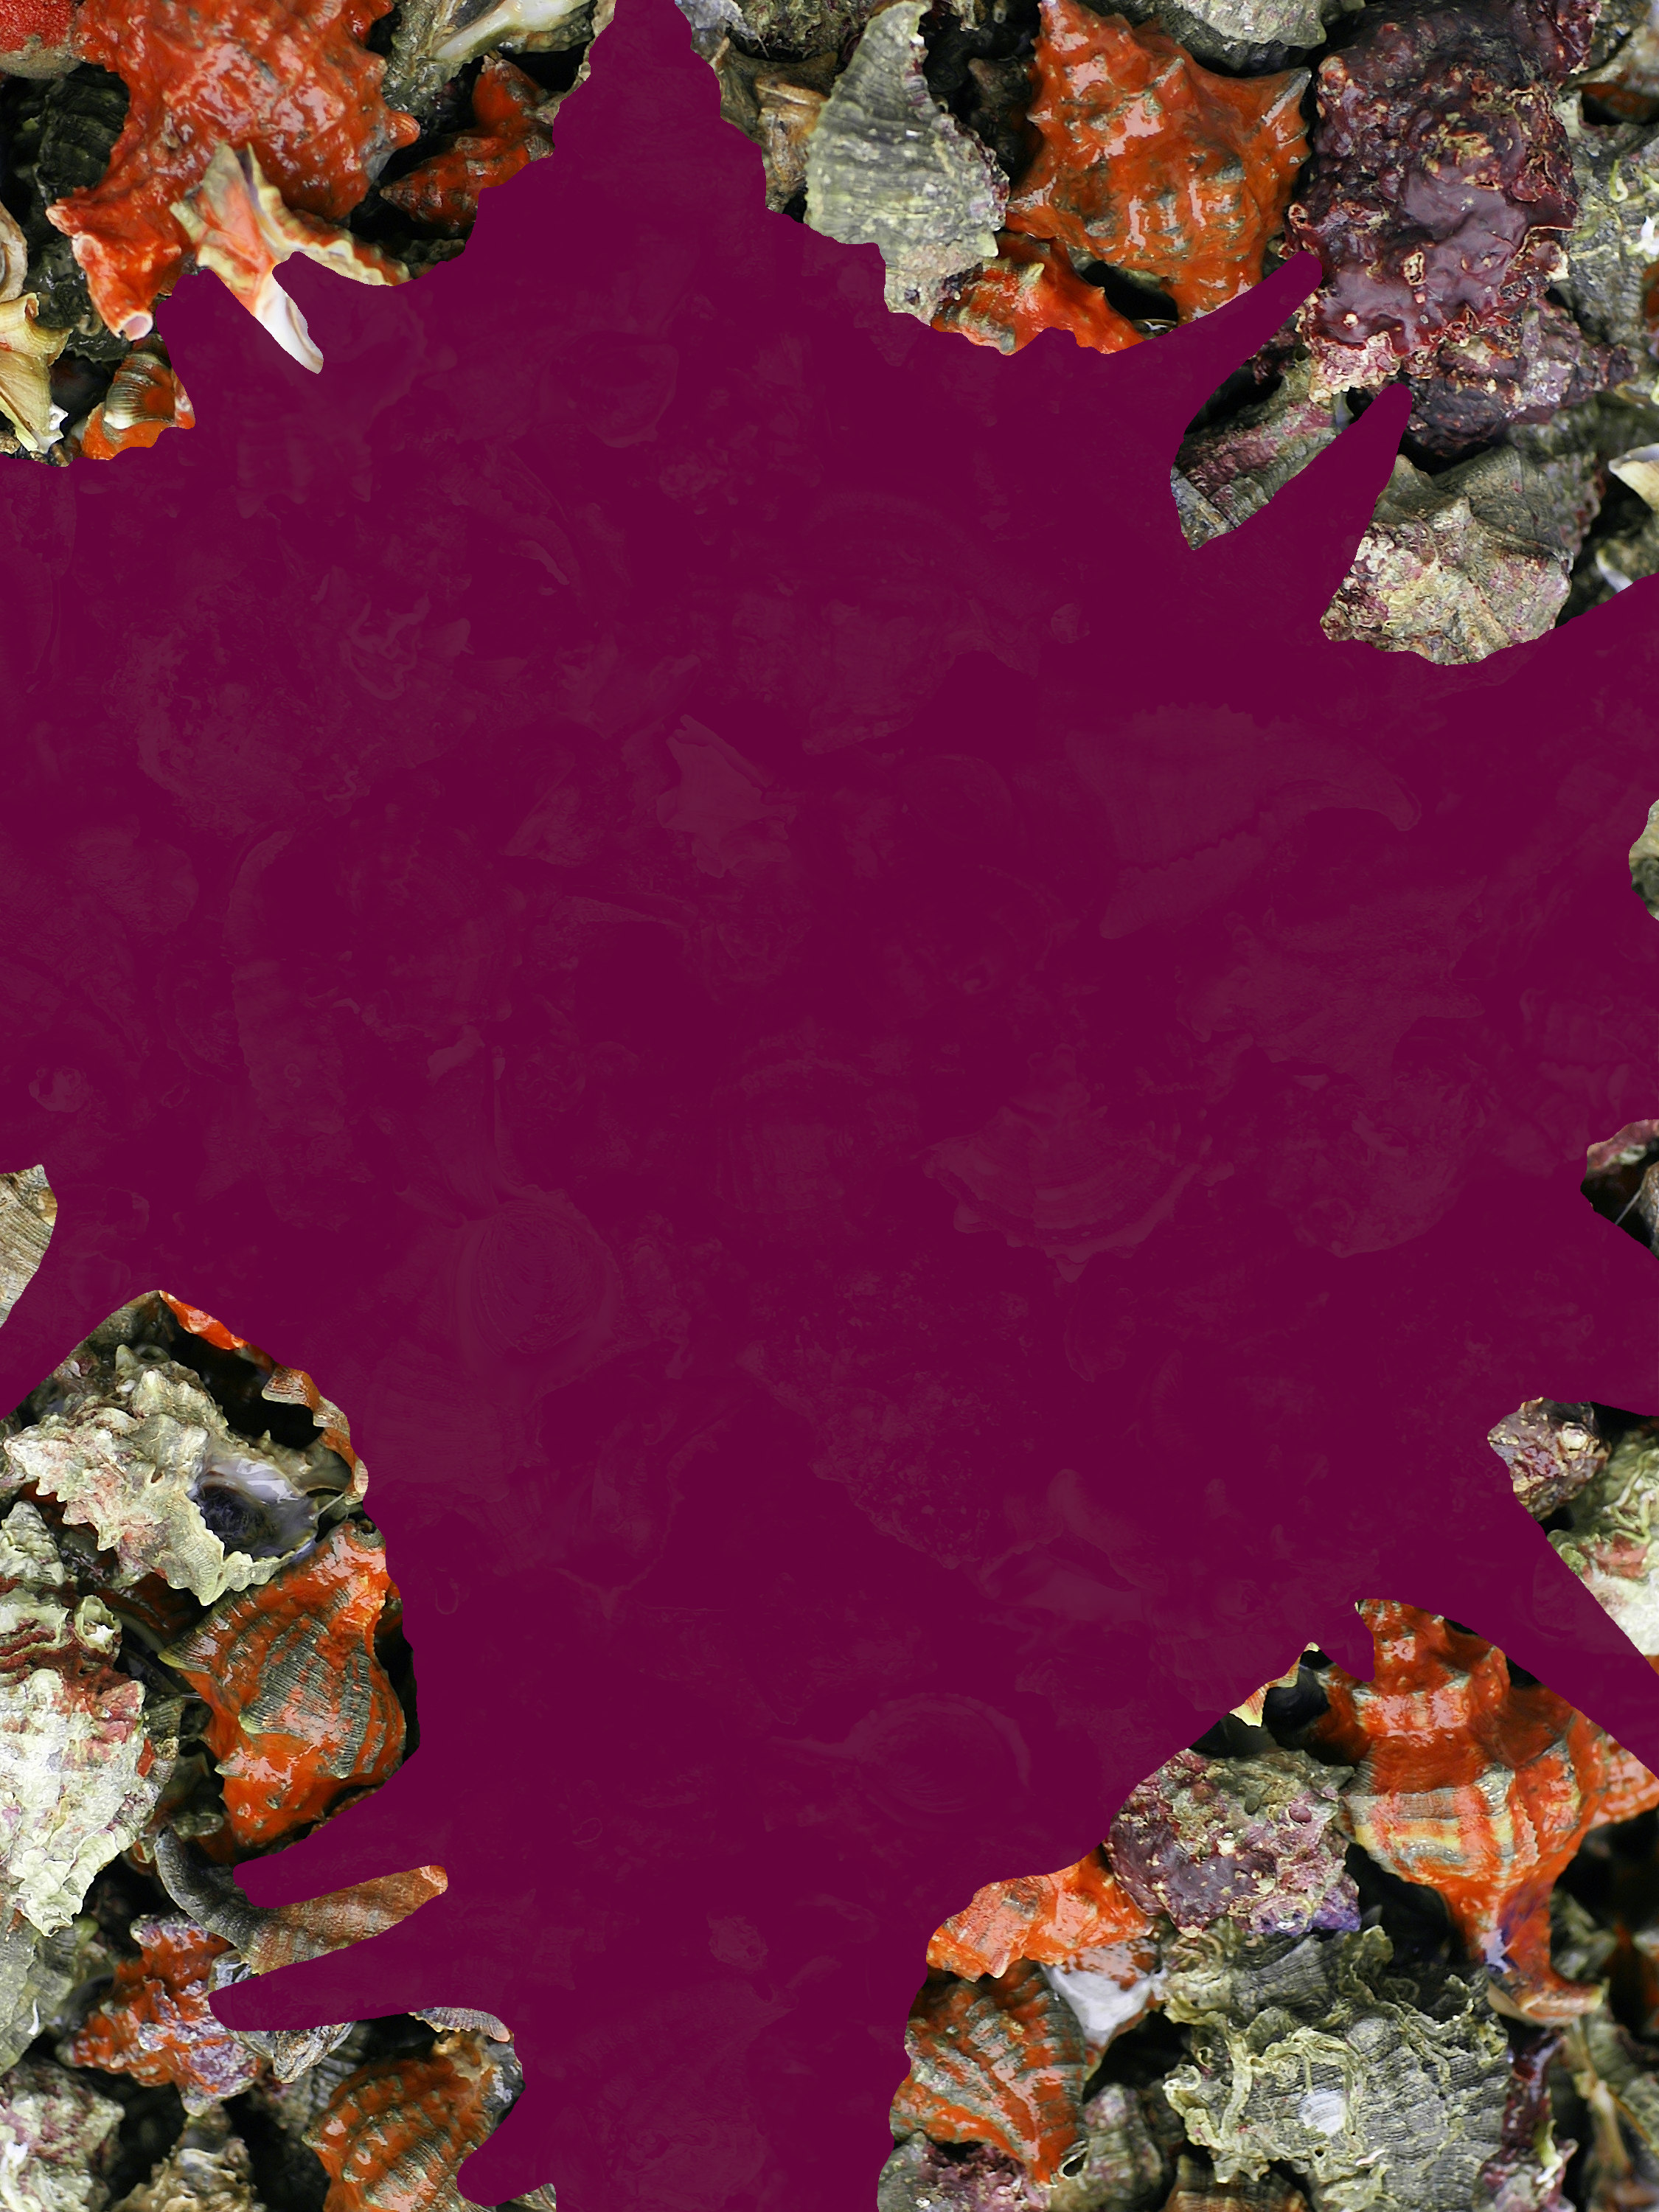
\includegraphics[width=\paperwidth,height=\paperheight]{murexpurple.jpeg}}
\begin{titlepage} % Suppresses headers and footers on the title page
	\centering % Centre everything on the title page
	%\scshape % Use small caps for all text on the title page

	%------------------------------------------------
	%	Title
	%------------------------------------------------
	
	\rule{\textwidth}{1.6pt}\vspace*{-\baselineskip}\vspace*{2pt} % Thick horizontal rule
	\rule{\textwidth}{0.4pt} % Thin horizontal rule
	
	\vspace{1\baselineskip} % Whitespace above the title
	
	{\scshape\Huge Mémoire sur la Pourpre}
	
	\vspace{1\baselineskip} % Whitespace above the title

	\rule{\textwidth}{0.4pt}\vspace*{-\baselineskip}\vspace{3.2pt} % Thin horizontal rule
	\rule{\textwidth}{1.6pt} % Thick horizontal rule
	
	\vspace{1\baselineskip} % Whitespace after the title block
	
	%------------------------------------------------
	%	Subtitle
	%------------------------------------------------
	
	{\scshape Par \Large M. Henri de Lacaze-Duthiers} % Subtitle or further description
	
	\vspace*{1\baselineskip} % Whitespace under the subtitle
    
	%------------------------------------------------
	%	Editor(s)
	%------------------------------------------------
        \vspace*{\fill}

	\vspace{1\baselineskip}

	{\small\scshape Paris 1860}
	
	{\small\scshape{Chez Derache, Rue du Bouloy N.° 7, au Premier}}
	
	\vspace{0.5\baselineskip} % Whitespace after the title block

        \scshape Internet Archive Online Edition  % Publication year
	
	{\scshape\small Utilisation non commerciale --- Partage dans les mêmes conditions 4.0 International} % Publisher
\end{titlepage}
\setlength{\parskip}{1mm plus1mm minus1mm}
\clearpage
\tableofcontents
\clearpage
\section{Ce qui a conduit à s'occuper de la question.}
\paragraph{}
Dès longtemps la question de savoir comment les anciens se procuraient la belle couleur qui fut dans l'antiquité l'apanage des grands et des rois a préoccupé les naturalistes ; ce n'est donc pas une question nouvelle dont il s'agit ici. Bien souvent la solution des problèmes dont l'intérêt, au point de vue de l'application, a complètement disparu, est due à une simple curiosité. J'avoue que c'est poussé par la seule curiosité de savoir avec quoi on produisait cette belle couleur que j'ai fait quelques recherches ; d'ailleurs, au point de vue anatomique, il faut reconnaître que ce que l'on trouve dans les ouvrages est bien vague, si même on trouve des renseignements exacts.

Tantôt, en effet, on rencontre dans les traités de malacologie les expressions \emph{poche à pourpre}, la \emph{veine à matière pourprée}, le \emph{réservoir}, etc. ; on va même jusqu'à dire que c'est la \emph{bile de l'animal}\footnote{Voyez Mémoire de M. Sacc, \emph{Bulletin de la Société industrielle de Mulhouse}, n° 130, 1856, p. 306. « Il est positif qu'à Tyr en préparait la laine en l'imprégnant d'abord du suc verdâtre d'un coquillage, et qui semble en avoir été la bile. »} ou \emph{suc pris de l'estomac} ; la coquille elle-même a été considérée comme fournissant la couleur.

Quand on s'occupe sérieusement de l'anatomie d'un groupe, on se contente moins facilement de renseignements aussi vagues ; et, il faut le dire, ce ne serait pas être difficile que d'être satisfait par cette série d'indications aussi peu précises que variées.

J'avais toujours le désir de m'occuper de la détermination exacte de l'organe producteur, mais je laissais cela, entraîné par d'autres occupations; d'ailleurs, après avoir fait quelques recherches bibliographiques, j'avais compris tout d'abord que l'on était loin de s'entendre sur l'espèce produisant la couleur. Et je ferai remarquer à cette occasion, que, tandis qu'il y avait doute pour moi lorsque je cherchais quelles espèces avaient employées les anciens, aujourd'hui ce doute a disparu ; cela tient à cette circonstance (on ne devrait jamais l'oublier, quand on veut interpréter les auteurs anciens), qu'il faut toujours mettre en regard des textes les résultats de l'observation directe de la nature. D'abord je n'avais pas fait de recherches précises sur les animaux eux-mêmes ; maintenant les espèces produisant la pourpre me sont familières ; quelques-unes n'ont pas changé depuis les anciens, les noms seuls ont été intervertis.

Une occasion s'offrit et me conduisit à faire les recherches que je présente ici.

Dans l'été que je passai en 1858 à Mahon, j'avais, ainsi que je l'ai dit à propos de la Bonellie, un pêcheur que le consul français, M. Walz, dans son obligeante protection pour les Français, m'avait procuré. Pendant que je fouillais les anfractuosités du port, Alonzo le plus souvent m'attendait dans sa barque ; parfois il employait les loisirs que lui laissaient mes recherches au bord du port à marquer son linge et ses vêtements ; ses culottes de toile blanche lui servaient de fond sur lequel il dessinait tant-bien que mal quelque croix ou quelque petit ange gardien.

Quand je le questionnais, il me répondait : « C'est pour ne pas égarer ou changer mes hardes avec celles des autres pêcheurs que je les marque ainsi. » Les traits formés par sa petite baguette de bois étaient jaunâtres. « Il n'y paraîtra guère ? lui disais-je. --- Ce deviendra \emph{colorado} (rouge), me répondait-il, quand le soleil l'aura frappé. » Il trempait son morceau de bois dans la mucosité du manteau déchiré d'une coquille, qu'il était facile de reconnaître pour la Pourpre à bouche de sang (\emph{Purpura hæmastoma}), et qu'il nommait \emph{cor de fel}.

Intrigué, je le priai de faire sur le tissu de mes vêtements, et sous mes yeux, quelques-unes des lignes et dessins qu'il savait exécuter ; puis, je continuai mes recherches ; mais bientôt je fus poursuivi par une odeur horriblement fétide, des plus pénétrantes, et, en observant les parties marquées, je vis une fort belle couleur violette d'une vivacité remarquable. Alonzo avait raison.

La pratique, en m'instruisant, me fournissait l'occasion de faire quelques études, et j'appris bientôt que, dans le port de Mahon, on trouvait le \emph{Cor de fel}, la Pourpre bouche de sang, en assez grande quantité. Il arrive rarement, lorsqu'on se trouve en rapport avec les pêcheurs, et si l'on peut parvenir à les faire converser, de ne pas apprendre quelque chose au milieu des erreurs, dont il faut savoir faire la part. On apprend toujours des choses justes, exactes, qu'il faut, il est vrai, interpréter et rapporter à leur véritable cause, ou bien dégager de ces exagérations que perpétuent, soit l'ignorance, soit la tradition de cette pratique qui sait tant et qui ignore bien davantage ; de cette pratique qui ne veut pas de la théorie, sans doute parce qu'elle redoute de savoir moins qu'elle, et qui cependant, si elle la consultait plus fréquemment, éviterait bien des erreurs, et ferait souvent de bien plus rapides progrès ; car l'une et l'autre se fournissent réciproquement des renseignements précieux, renseignements qui, certainement, les conduiraient toutes les deux plus vite à la vérité. Mais malheureusement il y a entre elles une répulsion bien difficile à vaincre, et cela non seulement quand il s'agit de la nature, mais encore pour toutes les autres branches de la science.

Les premières observations sujets de ce mémoire ont donc été faites à Mahon ; je les ai continuées à Lille avec des animaux que je devais à l'obligeance de M. Alfred Lejourdand, sous-directeur du jardin de zoologie de Marseille ; ses soins, aussi habiles qu'empressés, m'ont permis de recevoir une bourriche d'animaux venant de la Méditerranée en très-bon état ; je lui en dois mille remercîments, et j'ai terminé mon travail à Pornic, dans la haute Bretagne, à la Rochelle et à Saint-Martin-en-Ré, après avoir encore étudié dans mon laboratoire de la Faculté des animaux que j'avais recueillis à Boulogne-sur-Mer.
\clearpage
\section{Historique de la question.}
\paragraph{}
La Pourpre a disparu comme matière tinctoriale depuis longtemps ; ce n'est que dans quelques localités, fort arriérées sans doute que, d'après quelques auteurs,\footnote{Gonfreville, cité par M. Sacc, \emph{Société industrielle de Mulhouse}, n° 130, 1856, p. 107.} elle serait encore employée.

Son histoire doit donc être et se trouve en effet dans les ouvrages anciens. On sait que sa valeur était grande, et que son nom était employé pour désigner tantôt la royauté, tantôt la puissance : en latin, les \emph{Purpurati}, expression tirée de la possibilité de porter un habit de pourpre, servait à désigner les grands. C'était l'adjectif \emph{purpuratus} (qui porte un habit, des ornements couleur de pourpre), pris au pluriel substantivement. La valeur en était si grande que, s'il faut s'en rapporter à Théopompe, dont Athénée cite un passage dans son douzième livre, la Pourpre se vendait en Asie au poids de l'argent.\footnote{V. Athénée : ἰσοστάσιος γὰρ ἧν ἡ πορφύρα πρὸς ἀργυρὰν ἐξεταζομένη. (Athen. \emph{Deipnos.}, 12, c. 31, édit. Bipont., vol. 4, p. 455). --- Voyez aussi plus loin la note accompagnant un passage de Pline, où les prix sont indiqués en valeur de notre monnaie.}

Mais, de nos jours, les progrès de l'industrie ont fait perdre presque entièrement la valeur à cette matière tinctoriale. Aujourd'hui, dans de rares pays, tout au plus est-elle restée le secret de quelques personnes qui s'en servent pour marquer le linge, car elle est à peu près indélébile. Les choses sont donc bien changées depuis les temps anciens ; aussi ne trouvons-nous relativement à elle que des recherches de pure curiosité dans les temps modernes.

Dans les temps anciens, Aristote et Pline s'en occupent, comme on le pense bien ; l'un et l'autre font connaître comment on préparait la couleur. Il y aura lieu de revenir sur les faits que rapporte Pline, car on sait que cet auteur semble faire recueil des particularités les plus étranges : on croirait parfois qu'il s'impose de rapporter toutes les traditions, quelle qu'en soit la valeur ; il semble les accumuler à plaisir.

Il paraît préférable de juger les opinions diverses au fur et à mesure que les faits se présenteront. Pline et Aristote nous serviront beaucoup pour résoudre certaines questions ; on peut donc laisser de côté, pour le moment, leur texte et leurs opinions, dont l'interprétation se trouvera singulièrement simplifiée par l'exposé des faits que fournit l'expérience.

Les mémoires relatifs à la pourpre sont extrêmement nombreux, et l'on en trouve à peu près dans toutes les langues.

C'est surtout la recherche de l'espèce de coquillage employé par les anciens, et des procédés mis en usage par eux, qui sert de thème. Sans examiner tous ces travaux comme dans une revue critique, j'indiquerai cependant les principaux, et je choisirai surtout les points douteux qu'ils ne résolvent pas.

Bernard de Jussieu et Réaumur s'occupèrent de la Pourpre, et firent quelques expériences curieuses.

Il est assez intéressant d'étudier le mémoire de Réaumur ; on y trouve un enseignement qu'il est sans aucun doute utile de mettre en lumière.

Réaumur avait été sur les côtes du Poitou pour se livrer à différentes recherches, ainsi qu'il le raconte. On trouve son travail dans les \emph{Mémoires de l'Académie royale des sciences}.\footnote{Année 1711, p. 168.} Il avait, dans ses excursions au bord de la mer, exprimé sur ses manchettes le liquide de la Pourpre (qu'il désigne sous le nom de Buccin). Comme cela lui est habituel, il nous fait participer à l'étonnement que lui fait éprouver la découverte du développement de la couleur pourpre ; il porta surtout son attention sur les capsules que produisent les Pourpres, et où elles enferment leurs œufs : il reconnaît très bien que ces grains, ainsi qu'il les appelle, n'étaient autre chose que les œufs de son \emph{Buccinum}. Le liquide contenu dans ces capsules jouissait de la propriété de devenir pourpre comme une partie du tissu de l'animal.

Mais voici le fait qu'il semble utile de faire ressortir : il montrera combien, dans les sciences, quand le point de départ n'est pas juste, on dévie facilement ; combien surtout on arrive à des conclusions exactes en apparence, mais d'autant plus erronées, que les prémices ont été plus fausses et le raisonnement conduit par un homme plus habile.

Répétant chez lui les expériences qu'il avait faites sur ses manchettes en parcourant les grèves, Réaumur fut frappé de ne point voir se développer la couleur pourpre. Il s'approcha de la fenêtre, et bientôt il vit le violet qui s'était produit à la mer se représenter. D'où venait que dans le fond de la chambre la couleur n'apparaissait pas ? D'où venait qu'elle se montrait près de la croisée ?

« Je savais bien qu'il n'y a pas de moyen plus propre pour faire prendre promptement la couleur pourpre à la liqueur des \emph{Buccinum}, que d'exposer cette liqueur à un grand feu ou à un soleil ardent ; mais je savais aussi que le soleil n'avait point paru pendant tout le temps que j'avais été au bord de la mer. La chaleur n'avait donc point eu de part au succès de l'expérience que j'avais faite alors. »

Voilà certainement le point de départ de ses interprétations, qui sont complètement opposées à la vérité. Réaumur cependant était habile observateur, scrutateur consciencieux, prudent par-dessus tout. Qui n'a admiré ses belles observations sur les insectes ! observations où tant de faits se trouvent réunis ; malheureusement trop souvent presque inutiles, si ce n'est même perdues pour la science, par cette imperfection si regrettable de la nomenclature zoologique à l'époque où il écrivait et observait.

Il cherche partout la cause du développement de la couleur violette. Tantôt il croit que ce peut être la chaux, et cela parce qu'il remarque que la couleur arrive quand il place la liqueur sur la muraille près de la croisée de son appartement ; mais il est obligé de renoncer à cette explication. Tantôt il considère le soleil agissant seulement comme agent de calorique, et il ajoute même\footnote{\emph{Loc. cit.}, p. 166.} qu'en concentrant la lumière à l'aide d'une loupe, la teinte pourpre se développe très-vite dans le point ainsi soumis aux rayons concentrés, et cependant, quand il était sur la grève, le soleil était caché.

La conclusion qui lui paraît forcée d'après cela est celle qu'il indique dans les termes suivants :

« La cause d'un changement si prompt était alors aisée à apercevoir et tout le monde tire sans doute la même conséquence que je tirai, savoir que, puisque mes linges avaient toujours conservé la couleur blanchâtre de la liqueur dont ils étaient imbibés, lorsque je les avais laissés au milieu de ma chambre, et qu'au contraire, au lieu, de cette couleur, ils en avaient une pourpre lorsque je les avais mis sur ma fenêtre, on ne pouvait attribuer ce dernier effet qu'à la différente manière dont l'air agissait sur eux dans l'une et l'autre circonstance ; qu'il était dans un plus grand mouvement dans celle où ils rougissaient que dans l'autre où ils gardaient la première couleur de la liqueur. Qui eût jamais pu deviner qu'un peu plus ou un peu moins de circulation d'air eût pu produire si vite un pareil effet ? car les fenêtres mêmes de ma chambre, au milieu de laquelle je laissais les linges, étaient ouvertes. »

Ainsi, parce que le jour où il fit les taches sur ses manchettes en étant à la plage, il vit la couleur, bien que le soleil fût caché, il arrive à admettre que c'est le mouvement de l'air, et il est si convaincu de cette influence, qu'il ajoute :

« Il arrivait même, lorsque j'exposais les linges au grand air dans le milieu de la cour, et que, pour empêcher le vent de les emporter, je posais quelques petites pierres sur les coins, que tous les coins sur lesquels ces pierres portaient ne changeaient point du tout de couleur, quoique le reste prît une fort belle couleur pourpre.\footnote{\emph{Loc. cit.}, p. 176.} »

Et plus loin :

« C'est donc à l'air seul qu'il faut attribuer ce changement de couleur.\footnote{\emph{Loc. cit.}, p. 177.} »

Dans ce fait qui le frappe, à savoir, que les parties de ses linges qui étaient couvertes par les pierres ne se coloraient point, il y a toutes les propriétés photogéniques nettement indiquées, mais inaperçues ; tant il est vrai qu'un esprit souvent le plus supérieur peut faire erreur, par cela seul qu'il n'interprète pas, ainsi que cela doit être, une condition même des plus insignifiantes en apparence.

Réaumur, en faisant erreur et en attribuant au courant d'air ce qui devait simplement être rapporté à la lumière, a manqué, lui aussi grand physicien que naturaliste, la découverte (chose facile à reconnaître aujourd'hui) de la photographie. Cette manifestation si belle de la science moderne se traduisait à ses yeux par le fait de la couleur venue seulement dans les points non couverts par les petites pierres qui fixaient les pièces d'étoffes sur le sol de la cour ; mais il ne voit que le courant d'air, et l'action de la lumière ne lui apparaît pas. En remontant plus haut, bien avant lui indubitablement, on avait connaissance du fait ; car la couleur pourpre ne se développant que sous les rayons lumineux, il est impossible de pouvoir nier que les anciens avaient connu cette propriété. Seulement il fallait l'initiative ; il fallait cette idée qui s'applique à atteindre un but spécial ; il fallait cette simple pensée qui ouvre une nouvelle voie ; il fallait, en un mot, ce quelque chose qui, souvent bien longtemps attendu par les siècles, révèle toute une voie inexplorée, lorsqu'il est trouvé, crée une branche nouvelle que l'on dit ou croit être l'ouvrage d'un seul, alors que les générations ont accumulé les faits, et fourni les matériaux à celui qui a eu le bonheur de couronner l'édifice par un trait de génie qui paraîtra bientôt aussi simple que naturel.

Avant Réaumur, William Cole avait fait des essais tout à fait semblables.

On ne trouvera, du reste, dans les traités qui en font mention, rien qui puisse apporter une clarté quelconque relativement au sujet qui doit nous occuper.

De Jussieu avait opéré en 1709, Réaumur en 1711. Duhamel fit ses expériences en 1736. A bien des égards, il est le contradicteur de Réaumur. Lui aussi il s'occupe du changement de couleur ; il en décrit très-exactement les phases, il en indique la cause ; mais il finit par une explication peu conforme, sans doute, aux connaissances modernes.

Ayant montré comment Réaumur avait été conduit à une conclusion fausse, il est utile de rappeler les résultats du travail de Duhamel.\footnote{Voyez volume de 1736 des \emph{Mémoires de l'Académie des sciences}, p. 49.}

Si l'on voulait passer en revue tous les mémoires et écrits qui ont été publiés sur la Pourpre, on n'en finirait pas. Aussi, en appelant l'attention encore sur celui de Duhamel, le but est de montrer qu'il a fait des expériences qui auraient dû encore plus directement que celles de Réaumur le conduire à la photographie.

Duhamel fait remarquer que les changements de couleur sont très-connus ; il ne pouvait en être en effet autrement. Pline lui-même, dit-il avec raison, en fait mention. Le point qui fixe l'attention du savant est que l'action du soleil seule détermine la couleur. On a vu que Réaumur l'attribuait au renouvellement de l'air. « Ayant donc bien vérifié, par plusieurs expériences, que toutes les fois que je mettais le suc colorant de mes Pourpre sur du linge exposé au soleil, il devenait rouge en quelques minutes, après avoir passé par les couleurs dont j'ai parlé, je voulus m'assurer s'il ne prendrait pas cette couleur à l'ombre : pour cela je frottai un morceau de linge, que je laissai passer la nuit sur ma cheminée, mais il devint seulement vert, et ne rougit pas. J'essayai encore si le grand air ne réussirait pas mieux : pour cela, je mis de ce suc colorant sur un morceau de linge, que je posai sur ma fenêtre au nord, et sur laquelle la lune ne donnait pas, afin d'éviter toute lumière, et je le retirai le lendemain avant le soleil, il n'avait pas changé de couleur le jour suivant. Cette expérience prouve que le soleil agit d'une façon très singulière et très efficace sur le suc colorant dont il s'agit.\footnote{\emph{Loc. cit.}, p. 53.} »

Puis il recherche si le soleil a une action par la chaleur ou la lumière, en déterminant dans le premier cas une évaporation de quelque chose : « Je posai sur un appui de fenêtre bien échauffé par les rayons du soleil un morceau de linge mouillé du suc colorant, et que j'avais couvert en partie d'un écu ; dans ce moment, la partie du linge qui était exposée au soleil se colora, mais celle qui était sous l'écu resta seulement de couleur verte.\footnote{\emph{Loc. cit.}, p. 54.} »

Puis essayant la chaleur du feu, les résultats furent négatifs.

Voulant s'assurer que les corps couvrant les tissus imbibés n'agissaient qu'en interceptant les rayons lumineux, et non en empêchant une évaporation, il fit l'observation que, sous un verre épais de plusieurs pouces, la couleur venait aussi belle et très foncée.

Des papiers transparents de différentes couleurs, employés successivement, lui donnèrent des résultats curieux. On remarquera que sous un papier bleu, la teinte pourpre se développa bien. On sait que la couleur bleue est très-photogénique. « Mais ce qui me surprit le plus, dit-il, c'est que, quoique le papier bleu parût assez opaque, les échantillons qui étaient dessous étaient assez bien colorés.\footnote{\emph{Loc. cit.}, p. 53.} »

Ainsi se trouve démontrée l'action de la lumière aussi clairement que possible, et par cela même la fausseté de l'explication donnée par Réaumur. Mais Duhamel, lui aussi, avait fait des expériences démontrant les propriétés photogéniques ; il avait sous la main les phénomènes, base de cette science toute nouvelle, mais il n'avait pas trouvé l'explication. Celle qu'il donne n'est certainement pas à l'abri de tout reproche :

« Il me paraît que cette action du soleil sur cette liqueur est assez singulière, et mérite d'être examinée avec plus d'attention et de loisir que je ne l'ai pu faire, quoiqu'il paraisse qu'elle tienne assez à l'effet que cet astre produit sur les pêches, les pommes d'api, et quantité d'autres fruits qui ne prennent une belle couleur rouge que dans les endroits qui y sont exposés.\footnote{Voy. \emph{loc. cit.}, p. 59.} »

On trouve ici comparées deux choses qui ne sont guère comparables : dans un cas, c'est l'action des rayons solaires sur la matière soumise à la vie : dans l'autre, c'est cette même action sur des produits qui ont cessé d'être sous l'influence de la force vitale. Jamais le manteau des Pourpres ne se colore pendant la vie de l'animal : les mucosités seules prennent la teinte rouge violacé.

Par ordre de date, le mémoire que je citerai ensuite est de 1779 ; il est d'un Espagnol, et ne manque pas d'avoir assez d'intérêt. On y remarque aussi relatées les observations, comme les opinions des auteurs français et des autres naturalistes. L'auteur, don Juan Pablo Canals y Marti, inspecteur général pour S. M. \emph{del Ramo de la Rubia o Granza}, directeur général des teintures du royaume, est plein d'érudition et y traite à peu près de la plupart des questions relatives au changement de couleur de la matière, etc. Il y établit que beaucoup d'espèces peuvent servir à teindre ; que dans les Indes, comme dans l'Amérique, beaucoup de \emph{Caracols} (coquillages, limaçons) sont mis à profit par les teinturiers, et que les changements de couleur y sont connus.

Enfin il cherche à préciser d'une manière exacte la position de la partie de l'animal qui donne le produit propre à la teinture. Mais il n'est point anatomiste, et bien que, de tous les auteurs, ce soit celui qui donne une description des plus exactes, il ne traite nullement de la question qui doit surtout nous occuper ici.

Il ne m'est possible de citer quelques mémoires venus un peu plus tard que par des extraits que je trouve heureusement dans un auteur fort sérieux ; on verra plus loin les citations empruntées à l'auteur allemand auquel je laisse toute la responsabilité des faits qu'il avance.\footnote{Voy. plus loin \emph{Ann. des sciences nat.}, Zool. 4\textsuperscript{e} série, t. 12, citations de Heeren.} Quelle que soit la valeur de ces travaux, on peut prévoir cependant qu'ils n'ont pas dû traiter les questions de photographie et de structure, ainsi que la détermination de la partie productrice, en raison même de l'état de la science à leur époque, comme cela a pu l'être dans le présent travail. Du reste, il suffira de se reporter aux passages qui seront cités plus loin, pour reconnaître que Pline a servi largement, quand il s'est agi, soit de désigner les espèces, soit de faire connaître le prétendu réservoir de la Pourpre.

Aussi, Amati dans son travail \emph{De restitutione purpurarum},\footnote{Amati, \emph{De restitutione purpurarum}, 3\textsuperscript{e} édit. Cesena, 1784.} Capelli dans celui qu'il intitule \emph{De antiqua et nupera purpura},\footnote{Capelli, \emph{De antiqua et nupera purpura}.} et don Michael Rosa dans sa \emph{Dissertazione delle porpore e delle materie vestiarie presso gli antichi}\footnote{Don Michael Rosa, \emph{Dissertazione delle porpore e delle materie vestiarie presso gli antichi}, 1786.} ne doivent-ils pas s'être occupés de la question au même point de vue que nous. Tout en indiquant leurs travaux, je le répète, j'ai le regret de ne pouvoir en parler que d'après Heeren.

On lira avec le plus grand intérêt, et surtout avec beaucoup d'utilité, l'article \textbf{Pourpre} du \emph{Dictionnaire d'histoire naturelle} (1826), de M. Defrance ; on y trouvera, en effet, des traductions et des analyses, des extraits, pour les anciens, d'Aristote, de Pline, de Vitruve, d'Opien, d'Élien, de Pollux ; pour les modernes, de Belon, de Rondelet, de Gesner et d'Aldrovande, de Fabius Columna, de Guill. Cole, de Lister, de Réaumur, de Duhamel du Monceau, etc., etc.

Nous aurons à revenir sur quelques-unes des conclusions de cet article.

En se rapprochant beaucoup plus de ces derniers temps, on ne voit que deux travaux sur la Pourpre, l'un de M. Bartolomeo Bizio, l'autre de M. Sacc. On trouve bien aussi des dissertations critiques sur les interprétations des textes des anciens, des traductions d'Aristote et de Pline, et je puis en particulier citer celle que M. de Saulcy a fournie à M. Sacc, et qui a été publiée dans le même recueil que le mémoire du savant chimiste de Mulhouse.

Le travail de Bartolomeo Bizio a pour objet \emph{Investigazione chimiche sopra il Murex brandaris} Linn., et a été publié dans les \emph{Annali delle scienze del regno Lombardo-Veneto} (Padova, 1835).

Il y est question aussi du \emph{Murex trunculus}. Le travail est étendu, et la substance colorante semble avoir été traitée de toutes manières ; il y a des analyses fort nombreuses, ou plutôt des essais par les différents agents, eau, alcool, etc., des parties antérieures et postérieures du corps ou du corps tout entier ; il y a de nombreuses expériences sur la solubilité de la matière, sur l'action de l'ammoniaque, des alcalis, etc. Les analyses organiques laissent beaucoup à désirer, bien qu'il y soit parlé d'oxydation.

Je ne puis reconnaître s'il y a eu un principe immédiat isolé, et si cette question, fort intéressante, est résolue : \emph{La matière, avant l'action de la lumière, est jaune et non odorante ; après, elle est violette et d'une odeur des plus prononcées. Y a-t-il eu une transformation ?} Quelle est donc au juste la nature de l'action du soleil ? Quel changement a-t-il produit ? Quelle modification a-t-il imprimée à l'état moléculaire ou à la composition chimique de cette substance organique ?

Il était impossible que l'on travaillât, comme l'a fait Bizio, sur une pareille matière, sans reconnaître les changements de couleur sous l'influence des rayons solaires. Aussi ces changements sont-ils indiqués, de même qu'ils l'avaient été bien avant par Réaumur, Duhamel.

Bizio a extrait de la matière colorante un acide et un oxyde.

M. Sacc a publié dans le \emph{Bulletin de la Société industrielle de Mulhouse}, n° 130, année 1854, une esquisse de l'histoire de la Pourpre. Dans ce résumé assez succinct des travaux qui ont précédé son mémoire, M. Sacc s'occupe peu de la question anatomique ; il semblerait même qu'il n'a fait qu'une revue purement bibliographique, avec quelques rapprochements inspirés par les découvertes modernes relatives à l'alloxane et à la murexide. Il ne paraît pas, d'après ce travail, que M. Sacc ait fait d'expériences par lui-même. Son mémoire, du reste, lu à la Société industrielle, n'est pas long, et, comme tout ce qui est destiné à la lecture, est agréablement écrit, les faits y sont présentés d'une manière aussi claire que concise, et avec ce cachet apprécié par tous ceux qui connaissent l'éminent chimiste. Il y a cependant quelques-unes des conclusions qu'il n'est pas possible d'admettre, l'anatomie démontrant, par exemple, clairement que la partie productrice de la Pourpre n'est pas le rein, bien que cela soit affirmé, sinon d'après des expériences directes, du moins indiqué comme probable d'après l'analogie des couleurs que fournissent la matière à Pourpre et l'acide urique ou ses dérivés.

Dans leurs recherches historiques sur Rome et l'antiquité, il est rare que les auteurs ne parlent pas de la pourpre ; elle tenait un rang trop distingué parmi les couleurs des vêtements et les dignités, pour qu'un article ne lui soit pas toujours consacré. Or, le plus souvent, dans les citations bibliographiques, les auteurs se copient les uns les autres, en modifiant les expressions de leurs prédécesseurs suivant leur goût pour le style ; de là souvent des erreurs nouvelles faisant suite ou venant s'ajouter aux erreurs des textes que l'on prend pour guide.

On peut trouver, en histoire naturelle, bien des exemples de ces citations faites sans remonter à l'auteur original, et de ces citations tout à fait fautives qui se perpétuent de la sorte.

Parmi tant d'autres ouvrages où il est question de la couleur qui nous occupe, voici M. Desobry, dans ses \emph{Lettres}, du reste fort instructives et très-intéressantes, \emph{sur Rome au siècle d'Auguste, ou Voyage d'un Gaulois à Rome à l'époque du règne d'Auguste et pendant une partie du règne de Tibère}, qui donne aussi un extrait des auteurs, pour la faire connaître.

On trouve à chaque instant, dans les auteurs latins, \emph{tincta murice lana}\footnote{Horace.} ; les mots \emph{murex}, \emph{conchylium}, \emph{concha},\footnote{Voyez les dictionnaires classiques latins donnant des synonymies au mot \emph{Pourpre}. L'idée de coquillage y est bien établie ;\\\hspace*{5mm}« Quæ de Tyrio murice lana rubet. --- O. »\\\hspace*{5mm}« Purpura Thessalico concharum tincta colòre. --- Lr. »} reviennent bien fréquemment. C'est donc d'un coquillage qu'il est question dans Pline comme dans les autres auteurs, et, pour personne, un Limaçon de mer n'a été un Poisson. Et qu'on le remarque, ce n'est pas ici une distinction sévère, exacte et subtile d'histoire naturelle que je veux établir : non. Il n'est possible à personne de reconnaître un coquillage sous cette expression : « \emph{Un poisson de mer appelé Pourpre fournit cette riche teinture.} » Or cette expression, pour des personnes qui lisent simplement les ouvrages sans remonter aux sources, désignera bien ce qu'elle indique. Il est vrai de dire que si l'on ouvre un \emph{Gradus ad Parnassum},\footnote{\emph{Gradus ad Parnassum}, Quicherat, ouvrage classique.} on y trouvera, après le mot \textbf{Murex} : « \emph{Poisson dont on tire la pourpre} ; » après le mot \textbf{Pourpre} : « \emph{Couleur fournie par un coquillage que trouvèrent les bergers.} » Quel embarras pour celui qui n'est pas naturaliste, qui connaît seulement, comme tout le monde, que le Poisson n'est pas un coquillage, et réciproquement. Comment fixer son idée sur l'animal qui produisait cette belle couleur ?

C'est avec de telles traductions que, dans le tome 1\textsuperscript{er}, lettre 14, M. Desobry reproduit tout ce que dit Pline, avec des renvois en note indiquant le livre et le paragraphe. Mais pourquoi changer les expressions d'une manière aussi malheureuse : « \emph{Un poisson de mer appelé Pourpre fournil cette riche teinture}.\footnote{Desobry, \emph{loc. cit.}, p. 353, lett. 14 du tome 1.} »

Jamais Pline, au paragraphe 52, n'a parlé d'un poisson ; il a déjà fait assez d'erreurs pour ne point lui en faire commettre d'autres. Après avoir traité, dans le livre 9, des Crustacés, qu'il désigne par le nom de \emph{Cancer},\footnote{Voy. Pline, édition Panckoucke, t. 7, p. 78, 80, liv. 9, §§ 50, 51.} et des Oursins,\footnote{\emph{Ibid.}, p. 80, liv. 9, § 51.} il arrive aux Coquillages, et il dit en toutes lettres : « Viennent à présent les \emph{Murex}, dont les tests sont plus durs, et les divers genres de coquillages.\footnote{\emph{Ibid.}, p. 82, traduction de la collection Panckoucke, liv. 9, § 52, « Firmioris jam testæ Murices, et concharum genera. »} » D'ailleurs le mot \emph{couleur conchylienne} revient à chaque instant dans son ouvrage. Les erreurs se transmettent et se perpétuent par des citations incomplètes ou des changements de mots : c'est le cas ici. M. Desobry rapporte toutes les erreurs avancées par Pline, et ajoute celle qui vient d'être indiquée plus haut. Le Buccin lui-même y est désigné comme un « autre poisson de mer. » Déjà le texte est difficile à interpréter, quand on veut se rendre compte de l'espèce désignée par le naturaliste latin ; que devient-il pour celui qui prend l'expression \emph{poisson de mer} au sérieux ?

Dans tous les travaux, la propriété particulière à cette matière devait se trouver relatée. Il eût été curieux de faire des analyses organiques, et de voir, ainsi qu'il a été dit précédemment, ce qu'est cette matière. J'espère que mon excellent ami et collaborateur pour d'autres recherches de chimie physiologique, M. Alfred Riche, pourra m'aider à combler cette lacune, et que plus tard des notions exactes sur la substance trouveront leur place dans la science.

Ce qui est surtout l'objet du travail actuel, c'est la détermination exacte de la partie qui produit la matière colorante. Nulle part on ne trouve des données claires et nettes relatives à la question, et, après bien des recherches bibliographiques, il est encore possible de répéter l'une des conclusions que l'on trouve à l'article \textbf{Pourpre} du grand \emph{Dictionnaire d'histoire naturelle}.\footnote{Voy. \emph{Dict. d'hist. nat.}, t. 43, p. 235, art. \textbf{Pourpre}.} M. Defrance s'exprime ainsi :

« 5° Nous ne savons pas davantage au juste dans quelle partie de l'animal se trouve cette matière : est-ce dans l'organe dépurateur ? est-ce dans l'appareil-générateur lui-même ? Ce qui pourrait porter à le croire, c'est que les œufs du \emph{P. lapillus} contiennent la même liqueur en abondance, comme l'a observé Réaumur. Et alors on pourrait penser qu'il ne s'en trouve que dans les femelles, ce qui expliquerait l'observation de Duhamel, qui dit avoir vu des individus de la même espèce en avoir, et d'autres n'en avoir pas. »

Ces conclusions démontraient la nécessité de nouvelles observations, aussi est-il possible de présenter les faits qui suivent comme nouveaux et positifs.

Ayant eu à faire des recherches sur la matière pourprée, j'ai dû observer naturellement ses propriétés particulières : bien des auteurs en ont déjà parlé ; j'arrive un peu plus tard, alors qu'une nouvelle branche des arts, tirée de la science, est née, je veux dire la photographie, et j'ai pu mettre à profit cette découverte. Dans ces deux voies on ne rencontre rien, et c'est sur elle que j'appelle l'attention d'une manière plus spéciale.

En tout cas, on trouvera ici des notions précises qui permettront de voir nettement où est le lieu qui fournit la matière, et qui pourront conduire peut-être d'autres plus favorisés à pousser plus loin l'étude de cette partie de l'histoire des sécrétions dans les Mollusques. Ainsi se fait la science ; chacun apporte, suivant ses forces, ce qu'il peut, et le faisceau se constitue lentement et peu à peu, mais aussi sûrement ; mieux vaut dire moins, mais dire sûrement sans hypothèse. La bibliographie y gagne des notions précises, au lieu de ces opinions vagues, souvent contradictoires, qu'il faut contrôler, et qui nuisent sans aucun doute au progrès ; car le travail pénible rebute, et rien n'est aujourd'hui rebutant comme cette série de noms à citer, auxquels se rapportent trop fréquemment des opinions qu'on doit combattre.
\clearpage
\section{Des propriétés de la matière.}
\paragraph{}
Quand on enlève la matière qui doit devenir pourpre du lieu où elle se trouve, et dont la place sera plus tard assignée exactement, elle est blanche ou légèrement jaune. Dans le \emph{Purpura lapillus}, elle varie entre le blanc mat et le jaune. Dans la Pourpre hémastome, de même dans les \emph{Murex}, la teinte est parfois un peu grisâtre. Soumise à l'action des rayons solaires, ainsi que les anciens le savaient déjà très bien, ainsi que Réaumur l'a dit, et, après lui Bozio, etc., ainsi que les pêcheurs des côtes de la Méditerranée le savent par tradition, elle devient d'une teinte d'abord jaune-citron, puis jaune verdâtre ; elle passe au vert ; enfin elle vire au violet, qui se fonce de plus en plus, à mesure que l'action se prolonge davantage. On trouvera plus loin, lorsqu'il s'agira de déterminer exactement de quelle couleur devait être la pourpre des anciens, plus de détails et d'explications relativement à ce changement de couleur.

En étendant sur un tissu cette substance en couches de diverses épaisseurs, on peut avoir un violet foncé qui offre les tous les plus vifs, les plus riches, et parfois arriver au sombre le plus intense, ou bien enfin à la nuance la plus délicate.

En variant la quantité de matière et la durée de l'exposition au soleil, on peut arriver à faire des dessins qui ne manquent pas, avec une grande vigueur de ton, des teintes dégradées les plus douces.

Une matière qui se comporte de la sorte mérite aujourd'hui, à coup sûr, le nom de \emph{matière photogénique}, et il était donc tout naturel de faire des essais dans cette nouvelle voie.

Quand se trouveront exposées, ainsi que cela aura lieu bientôt, les propriétés des tissus, les connexions de la glande ou de la partie productrice, il sera plus facile de juger du parti que peut-être on pourrait tirer, au point de vue de la science et même de la pratique, des propriétés de la pourpre. Mais voyons d'abord quels résultats on peut obtenir.

En recueillant la matière purpurigène à l'aide d'un pinceau un peu rude, que les peintres nomment \emph{brosse plate}, dont on coupe et raccourcit les crins, on arrive très bien à se procurer toute la quantité produite par un animal. Il suffit pour cela de brosser tout doucement plusieurs fois, sans se lasser, la partie qui sécrète. Bientôt la brosse se trouve chargée d'une substance visqueuse et filante qui reste adhérente. Alors on n'a qu'à barbouiller les tissus que l'on veut imprégner, en répétant fréquemment sur eux un mouvement de moulinet ou de va-et-vient. On arrive ainsi à étendre en couche uniforme la mucosité recueillie, qui fait d'abord un peu de bave ou de mousse, mais qui bientôt ne forme plus qu'un liquide, quoique épais, où toutes les bulles d'air disparaissent progressivement. Pour que le tissu se trouve imprégné à peu près uniformément, on charge le pinceau une seconde, une troisième, une quatrième fois, en ayant soin de bien fondre les limites des différents points sur lesquels on apporte successivement de la nouvelle matière.

Pour réussir à avoir une couche de matière uniforme sur l'étoffe, on doit employer d'abord la brosse ; puis, passant le doigt en différents sens, on doit chercher à faire cheminer, des points plus imbibés vers les creux qui le sont moins, l'excès de matière.

Tantôt j'ai opéré presque au grand jour, tantôt dans l'obscurité ; je dois dire que dans ce dernier cas j'avais peut-être plus de détails. Cependant j'ajoute que la matière n'étant point encore modifiée donnait, quand je la préparais au jour, des résultats encore très satisfaisants.

Je laisse de côté toutes les minutieuses précautions qui sont bien connues de tous les photographes, et qui n'ont rien de spécial, quelle que soit la matière photogénique employée. Bien faire adhérer le tissu chargé de la couche photogénique au cliché qui doit être reproduit ; éviter les bulles d'air, etc., etc., tout cela étant connu, et n'ayant rien de particulier, peut être laissé de côté.

Il faut un certain temps au soleil, même avec un cliché négatif, pour obtenir une épreuve positive ; par conséquent, il serait infiniment plus long d'avoir une épreuve dans la chambre obscure par l'action simplement de la lumière réfléchie. Je n'ai pris qu'une image d'un objet, sur lequel, à l'aide d'une glace, tombait la lumière directe du soleil. Le tissu exposé dans la chambre obscure a présenté l'image, ainsi qu'il était facile de le prévoir.

Le temps nécessaire au développement de l'image positive varie avec la vivacité des rayons lumineux du soleil. On observe surtout très-bien le passage des tons divers, quand on soumet la matière à la lumière solaire, masquée de temps en temps par des nuages, la durée de l'expérience étant alors beaucoup plus longue. Une image était reproduite à Pornic (Vendée), à la Rochelle (Charente-Inférieure), à Agen (Lot-et-Garonne), en quatre ou cinq minutes, par un beau soleil, et cela vers la mi-août, fin du même mois et le commencement de septembre. Dans cette dernière localité, un portrait n'était fini qu'après trois quarts d'heure par un ciel nuageux, mais laissant encore entrevoir de temps en temps de très-pâles rayons de soleil.

Je n'ai point calculé le temps nécessaire au développement de la couleur à Mahon, mais il me paraissait infiniment plus court : deux minutes, une minute même, ont quelquefois paru suffire, autant que je puis comparer par souvenir un temps non calculé à un temps dont la durée a été bien appréciée. Mais le ciel dans les îles Baléares est si lumineux, la lumière y est si vive et le soleil si pénétrant, que cela doit être et ne peut étonner.

Avec des clichés négatifs, on obtient des portraits pleins de vigueur et de netteté, qui présentent les caractères dus aux changements successifs de couleur de la matière.

Pour que la matière passe successivement aux teintes indiquées, il faut qu'elle soit constamment mêlée à une certaine quantité d'eau. Après avoir étendu la pièce de tissu sur la plaque portant le négatif, il est bon de l'humecter avec quelques gouttes d'eau de mer, puis d'appliquer une étoffe, également humide, ployée en plusieurs doubles ; on recouvre le tout avec une seconde plaque, et l'on expose au soleil. Il faut aussi, quand la chaleur est grande, avoir soin d'ajouter de temps en temps quelques gouttes d'eau, afin que le contact de la pièce chargée de matière reste constant et parfait ; sans cela, le tissu s'isole un peu de la plaque négative, des bulles d'air se forment et nuisent à la pureté de l'image.

En ajoutant ainsi de l'eau, on observe le derrière du tissu, et l'on juge de l'état de développement des couleurs et des tons.

Pour arriver à avoir des ombres bien accusées, ordinairement on doit suspendre l'insolation quand les parties qui doivent être blanches dans les images obtenues par les matières photogéniques ordinaires présentent ici une belle teinte jaune verdâtre. Si le vert est trop accusé, les violets envahissent tout, et les jaunes ne font plus assez de contraste avec les violets représentant les noirs qui ne sont pas foncés en proportion.

Dans les images ainsi obtenues, on trouve donc les noirs remplacés par une teinte violette d'autant plus foncée que la lumière solaire a pu mieux traverser la photographie négative. Cette teinte violette se dégrade successivement, et passe au jaune d'autant moins intense et moins verdâtre surtout, que les noirs sont plus accusés dans le négatif. C'est aussi ce qui m'a fait choisir, pour faire des épreuves positives, des clichés fort accentués et présentant des contrastes de noir et de blanc très-tranchés.

La teinte et les reflets que présentent ces photographies sont fort agréables, et sur une reproduction de la tête d'une vieille femme, la nuance du jaune pâle formant les blancs de la figure imitait assez la teinte de la carnation de la vieillesse. D'ailleurs, il y a, comme on peut le remarquer, harmonie de couleur, le jaune et le violet étant complémentaires l'un de l'autre.

Sans aucun doute, avec des espèces donnant une grande quantité de matière purpurigène, on obtiendrait plus facilement une couche égale et uniforme ; car les temps d'arrêt, qui sont la conséquence de la recherche de la matière sur plusieurs petits individus, comme le sont ceux du \emph{Purpura lapillus}, se font souvent plus ou moins remarquer par quelque inégalité de la couche impressionnable. Il est en effet, assez difficile de reprendre juste dans le point où l'on a cessé d'étendre, et alors les traits ou les décroissances de teinte se trouvent plus ou moins accusées, suivant qu'il y a plus ou moins de matière.

Sur papier, on aurait des épreuves ayant infiniment plus de détails et de vigueur ; mais la difficulté se trouve dans l'impossibilité où l'on est de pouvoir agir avec une brosse ou un pinceau dur pour étendre la matière impressionnable. Quelques essais n'ont pu être faits qu'à la condition d'étendre la substance avec le doigt sans trop frotter afin de ne point enlever le poli de la feuille de papier.

Je ne doute pas que l'on n'obtienne de très-bons résultats sur papier ; mais n'ayant, dans mon dernier voyage au bord de la mer, que peu de clichés, et l'adhérence qui s'établissait entre le papier et le collodium me faisant redouter d'enlever ce dernier, j'ai renoncé à continuer les essais, dans la crainte d'être obligé de cesser mes expériences. Mais, évidemment, le tour de main consisterait à imprégner le papier sans l'érailler ; or, je crois volontiers qu'on arriverait facilement à le trouver.

A quel usage pourrait-on employer la pourpre ?

Aujourd'hui que les manufactures de produits chimiques versent à torrent dans l'industrie des matières qui, avec la plus grande facilité et la plus grande perfection, peuvent servir aux teintures les plus délicates et les plus riches, comment pourrait-on espérer de voir ce peu de matière animale donnant du violet, quoique fort beau et fort tenace, être employé par l'industrie ? Il n'est guère probable que la pourpre revienne en honneur.

Toutefois, il me paraît utile d'appeler l'attention sur un point : la photographie n'a pas encore tourné ses efforts vers l'application sur les étoffes délicates des dessins et des peintures d'un fini comme elle en fait. On a bien, il est vrai, sur certaines toiles cirées, appliqué la couche de collodium déposée sur une glace et portant une image ; mais on n'a pas, par exemple pour des éventails et tout autre objet de luxe très délicat, donné sur soie des reproductions des dessins, des tableaux, etc., que la photographie procure avec la plus grande facilité.

On peut donc se demander si, en étudiant avec soin la matière purpurigène, si en arrivant à dissoudre la matière restée jaune quand on a fait la photographie, on ne pourrait utiliser ces reproductions sur soie ayant cette belle teinte violette dont il a été question. Il serait facile alors de pouvoir utiliser sous forme de médaillons, sur les pages et les cartons de tel ou tel de ces petits objets de luxe, un portrait ou une scène prise aux grands maîtres reproduits avec cette facilité et cette fidélité que chacun connaît au daguerréotype.

C'est là sans doute une application fort restreinte ; mais cependant, quand on voit la douceur des tons et les nombreux détails, ainsi que leur finesse, des photographies obtenues avec la matière des espèces indiquées plus haut, on se demande si, dans ces industries de luxe et d'objets si délicats à la mode, on ne pourrait utiliser cette propriété photogénique, qui permettrait de trouver un usage à cette matière si recherchée des anciens et si délaissée aujourd'hui.

La soie, d'ailleurs, conserve ce brillant et ces reflets qu'on lui connaît, et si l'on venait à employer ce moyen photographique, on obtiendrait de l'industrie des soies certainement avec un grain plus fin que celles qu'on trouve dans le commerce, et qui cependant donnent déjà de très-beaux résultats.

Les étoffes sont d'ailleurs fortement imprégnées de la matière colorante, et le dessin apparaît toujours également net et vif, quelle que soit la face du tissu que l'on examine. On a vu que la pourpre ne devait pas se faner ; on sait aussi que si elle perd d'abord un peu de son teint vif par le lavage, ensuite elle persiste ; on aurait donc des conditions de conservation très-bonnes, et qui donneraient peut-être plus d'importance qu'on ne le pense à cette branche de la photographie.
\clearpage
\section{Que se passe-t-il pendant l'action du soleil, et dans le changement de couleur ?}
\paragraph{}
C'est là une question qu'il est assez difficile, de résoudre sans des recherches de la plus grande délicatesse et des analyses organiques probablement fort difficiles, sinon fort minutieuses.

La première chose qui frappe est celle-ci : développement, conjointement et parallèlement à la production de la teinte violette, d'une odeur vive et très pénétrante, que bien des personnes, à qui je demandais inopinément, sans qu'elles fussent prévenues, --- quelle est cette odeur ? --- comparaient soit à l'odeur de la pierre à fusil, soit à l'odeur de la poudre brûlée, soit enfin à l'odeur de l'ail, de l'assafœtida. Les chimistes à qui j'ai fait la même question donnaient tous et toujours cette odeur comme étant celle de l'essence d'ail.

L'odeur est extrêmement pénétrante au moment où la couleur vient à se produire ; elle persiste encore pendant fort longtemps ; elle ne se reproduit toutefois que lorsque l'on humecte le tissu coloré. Cependant, après un certain temps, elle semble disparaître ; mais quand on la connaît bien, on la retrouve sur les tissus que l'on imbibe. Une petite pièce de batiste teinte en violet à Mahon, en 1858, au mois d'août, exhalait l'odeur d'une manière très forte en la lavant un an après.

Il se forme donc un produit, une matière nouvelle ; cela semble être une conclusion forcée, puisque les caractères physiques ont si complètement changé.

La matière non influencée par la lumière est certainement soluble dans l'eau et dans l'alcool. Les preuves de ce fait sont nombreuses. D'abord quand on laisse mourir un animal, non-seulement la partie renfermant la matière devient pourpre, mais les tissus environnants se colorent eux-mêmes : cela tient à ce qu'ils se sont imprégnés du liquide évidemment par imbibition, et ils deviennent également pourpres. Les bords du manteau sont sans aucun doute complètement dépourvus de matière influençable, et cependant, sur les animaux morts, on les trouve souvent d'un beau violet.

De plus, les animaux qu'on plonge dans les liquides conservateurs colorent la liqueur. J'ai placé dans des tubes avec de l'alcool des portions du manteau de la Pourpre hémastome, à Mahon ; l'alcool était devenu d'un beau violet.

Au Jardin des Plantes des Pourpres conservés dans les liquides, ont une partie du manteau d'un beau violet.

Cet effet s'est présenté constamment dans les flacons que j'ai.

Enfin, quand on ajoute des gouttes d'eau sur les linges imprégnés de la matière, l'eau qui s'écoule va teindre les parties environnantes d'une teinte légère. Evidemment il y a eu dans ce cas solution de la matière.

Plus tard, quand la matière est devenue violette, elle est parfaitement insoluble, et sa stabilité sur les tissus en est la preuve. Avant d'aborder de nouvelles questions, il est important de dire quelques mots sur la persistance de la teinte.

J'ai fait des marques et des dessins sur du linge ; en particulier, j'avais fait mes initiales sur le coin de l'un des mouchoirs qui me servaient dans mon voyage ; et encore, bien que ce mouchoir ait servi avec intention très-fréquemment, et que le tissu en soit rompu, les lettres de la marque sont encore d'un très-joli violet un peu pâle, mais cependant d'une teinte extrêmement agréable.

Du reste, l'habitude qu'ont les matelots de marquer leur linge avec le \emph{Cor de fel}, à Mahon ; leur opinion, qui est la même pour tous, savoir, que les marques resteront inaltérables, prouvent que la matière, une fois colorée ou transformée, reste toujours inattaquable.

Dans quelques essais que je faisais pour enlever la matière non attaquée, le chlorure de fer l'a détruite, mais le chlorure de chaux a agi beaucoup moins efficacement.

La potasse, l'acide acétique, l'ammoniaque, l'acide chlorhydrique, ne m'ont pas paru altérer ou même modifier la teinte.

La matière doit évidemment imprégner les tissus, et se modifier dans leur intérieur pour y rester ensuite indéfiniment. C'est ainsi qu'en enlevant la matière à pourpre avec une brosse, pour fournir un point d'appui au manteau, je le renversais sur mon pouce pour que les tissus pussent être brossés et dépouillés de leur matière. L'ongle était recouvert naturellement de matière ; il s'imprégnait tout à fait comme un tissu ordinaire, et conservait cette belle couleur pourpre plus de cinq semaines. L'ongle continuant à croître, la partie de nouvelle formation tranchait, après un certain temps, par sa couleur blanche sur la partie rouge antérieure. Évidemment, surtout quand on se livre à des recherches, quand on va à la mer presque tous les jours, voilà des conditions de lavage qui devraient faire disparaître vite cette teinte, si elle n'était fort tenace et fixée d'une manière presque indélébile : mais incorporée aux tissus et précipitée dans leur intérieur à l'état moléculaire, elle y reste fixée.

Ainsi voilà des propriétés remarquables : insolubilité, inaltérabilité, à la suite de l'action de la lumière.

La valeur qu'avait auprès des anciens la pourpre peut certainement trouver une raison dans ce fait : que, sous les climats brûlants et le ciel toujours si lumineux de l'Italie, de la Grèce et de l'Orient, la pourpre ne devait pas se faner comme les autres couleurs rouges, surtout comme celles tirées du règne végétal ou animal. La Cochenille, dont parle Pline,\footnote{Voy. Pline, t. 7, édit. Panckoucke, p. 115 et 114, liv. 9, § 65, traduction, etc. : « Quin et terrena miscere, coccoque tinctum tyrio tingere, ut fieret hysginum. Coccum Galatiæ rubens granum, ut dicemus in terrestribus, aut circa emeritam Lusitaniæ, in maxima laude est. »} et qui fournissait l'écarlate, ne devait point résister à l'action solaire. La pourpre, au contraire, qui a eu pour cause directe cette lumière même, ne peut s'altérer comme les autres couleurs. Évidemment tout ce qu'aurait pu faire le soleil, et les anciens étaient souvent exposés dans leurs cérémonies publiques à ses rayons, c'eût été de renforcer le ton des étoffes ; et l'on doit voir là certainement une des raisons de cette estime de la pourpre entre toutes les autres couleurs.

Quand on connaît ces faits, on ne peut se refuser d'admettre qu'il a dû se former un composé nouveau.

M. Sacc a dit dans son rapport : « Il est évident que la matière à pourpre est accompagnée par une autre matière qui joue le rôle de mordant, et c'est à ce mordant qu'est due la fixation de la couleur. »

Est-il absolument nécessaire, pour qu'une matière se fixe, qu'elle soit accompagnée d'un mordant ? Il y a bien des cas en teinture où l'on n'a pas besoin de mordancer les étoffes ; et ici je crois, sans m'être livré pour cela à des recherches particulières, qu'il y a pas de mordant. La substance est soluble, elle imprégné les tissus ; elle devient insoluble, se précipite, et reste par cela même fixée.

Il faut dire cependant que les parties environnantes du manteau sécrètent une mucosité assez épaisse qui se mêle toujours, et quoi qu'on fasse, avec la matière à pourpre. Ce mucus aide beaucoup à rendre la couche de matière parfaitement égale dans le cas où l'on veut faire des photographies. Mais il faut aussi savoir que, si l'on a une trop grande quantité de mucus, celui-ci forme une sorte de vernis, de couche superficielle, qui se colore d'abord, et qui forme écran à la surface de la matière imprégnée dans le tissu. Si donc on a fait une photographie en laissant un trop grande quantité de mucus, on a l'image à la surface, en dehors des tissus, ce qui fait que, pour peu qu'on humecte l'étoffe et qu'on la fasse adhérer à un autre tissu, on perd une grande partie de l'image.

Maintenant quelle est l'action de la lumière sur cette matière ? Et d'abord c'est une action de la lumière, et non autre chose.

On a vu quelle interprétation avait donnée Réaumur. Pour lui, c'était une action de l'air ; un renouvellement de ce fluide était absolument nécessaire pour produire la modification de la matière. Or non-seulement les expériences de Réaumur prouvent que c'est bien la lumière qui agit ; mais il suffit d'avoir fait une épreuve photographique quelconque pour se convaincre de la parfaite inutilité de ce renouvellement. Placée entre deux plaques de verre, il est difficile de trouver là pour la matière les conditions que disait nécessaires le grand observateur. Il n'est donc pas possible d'admettre l'action de l'air, au moins ainsi que l'entendait Réaumur.

C'est bien une action de la lumière, car les Pourpres placées dans des liquides conservateurs ne manquent pas de se colorer dans les points voisins de la place qui produit la pourpre : dans ce cas, il est difficile de voir une action de l'air ; sous l'eau, dans un flacon bouché, il n'y a pas de courant et de renouvellement. Ce qui ne prouverait encore rien relativement à un autre mode d'interprétation, car l'eau tient en dissolution une assez grande quantité d'air. Mais on a vu que déjà Duhamel avait combattu par des expériences décisives cette opinion.

Afin que les liquides imprègnent les animaux que l'on veut conserver, il est bon d'en briser la coquille. Dans un voyage, mon but étant d'obtenir simplement des animaux conservés pour servir au besoin, je jetais dans un flacon indistinctement les individus après en avoir concassé le test. Or, toujours les animaux dont la coquille était intacte restaient incolores, et les animaux dont la coquille était en partie brisée restaient blancs sous les fragments et s'empourpraient dans les parties qui voyaient la lumière.

Si donc l'action de l'air dissous dans l'eau alcoolisée était invoquée pour expliquer ce changement, il faut bien le dire, cette action ne pourrait être, sans aucun doute, accomplie que sous et par l'influence de la lumière.

Et il ne faut pas croire que ce soit seulement des rayons lumineux directs du soleil qui cause ce changement : la lumière diffuse le produit également ; mais l'action est beaucoup plus lente que lorsque les rayons du soleil agissent directement. Les flacons qui renfermaient les Pourpres concassées n'étaient certes pas exposés à la lumière directe, et cependant la couleur s'était développée.

Mais en quoi consiste cette action, et comment l'expliquer ? Des circonstances ayant porté obstacle aux recherches que nous devions faire avec M. Riche, j'avouerai que je ne poserai ici, pour ainsi dire, que des questions.

La première idée qui se présente est celle-ci. La matière subit sous l'influence du soleil une oxydation. Cette opinion n'est pas nouvelle ; il en est déjà question dans quelques-uns des travaux cités.

Ce qu'il y a de positif, c'est qu'il serait nécessaire de bien savoir ce qu'est la matière avant l'action de la lumière, et ce qu'elle est après. Sans aucun doute, il y a un produit nouveau de formé ; mais ce produit est-il le résultat d'une simple modification dans l'arrangement moléculaire, sous l'influence de cet agent profondément modificateur ? Sans analyse, il n'est guère possible d'en décider. Réaumur croyait déjà que la modification était toute moléculaire.

S'il y a oxydation, ce qui pourrait bien être, le produit nouveau est-il plus complexe ? Quel est-il, comparé ce qu'il était avant. Voilà certainement des recherches intéressantes, et qui, je l'espère, conduiront à des données exactes.

Quoi qu'il en soit, l'odeur qui se développe est parfaitement caractéristique, et, chose curieuse, elle se développe dans toutes, les espèces qui fournissent la couleur, que ce soit les \emph{Purpura hæmastoma} ou \emph{lapillus}, les \emph{Murex trunculus}, \emph{brandaris} ou \emph{erinaceus}, toujours l'identité d'odeur est absolue. Les personnes qui n'ont pas senti l'essence d'ail la comparent peut-être avec quelque raison à l'odeur du reste de la poudre qui a brûlé ; d'autres à celle un peu sulfhydrique que dégage du silex frappé ; on pourrait lui trouver de l'analogie avec celle que l'on sent quand une voiture marche avec un sabot à l'une de ses roues. Il y a aussi une très grande analogie avec l'odeur de l'ail et de l'oignon brûlés. C'est dans la constance de cette odeur qu'il faut surtout chercher une preuve de la formation d'un corps nouveau, soit qu'il y ait un changement de l'état moléculaire, soit qu'il y ait absorption de l'oxygène, et par conséquent production d'une combinaison nouvelle avec un plus grand nombre d'éléments.

Cette question sera, je l'espère, résolue plus tard, quand les analyses et les recherches que je ne puis entreprendre seul pourront être conduites par mon très habile ami et collaborateur.

Il serait à propos, après avoir parlé des propriétés de la matière et de sa ténacité, de dire un mot de sa teinte ; mieux vaut, pour éviter des répétitions, s'occuper de cette question quand il s'agira des espèces fournissant la couleur.
\clearpage
\section{Position de la glande ou partie produisant la matière à pourpre.}
\paragraph{}
Ainsi qu'il a été dit en commençant, le but principal de ce travail est la détermination anatomique exacte de la partie du corps des Gastéropodes fournissant la matière colorante.

--- Qu'est-ce donc que cette partie ? où est-elle placée ?

--- Est-elle particulièrement spéciale aux espèces donnant la matière colorante ?

--- La retrouve-t-on dans tous les Mollusques gastéropodes ?

Voilà tout autant de questions qu'il faut résoudre, et dont la solution permettra seule d'arriver à une détermination anatomique générale satisfaisante.

Où est située la partie fournissant la matière pourprée ?

Il me paraît à peu près inutile de citer les auteurs dont les indications sont les plus vagues et les plus entachées d'erreur. Les mots \emph{veine}, \emph{poche}, \emph{sac à pourpre}, doivent également et tout d'abord être rayés, leur emploi étant fautif.

Un des auteurs qui ont cherché à donner le mieux l'idée du lieu où il faut puiser la matière tinctoriale est Juan Pablo Canals y Marti, dont le mémoire a été déjà indiqué.\footnote{Voyez, à la fin de notre mémoire, la note relative au travail de MM. Grimaud et Gruby.} Il compare la coquille de la Pourpre à celle d'un limaçon de jardin, puis il fixé le point où se trouverait dans celui-ci les vases, les vaisseaux qui préparent la matière. La comparaison n'est peut-être pas très heureusement choisie, cependant elle sert à indiquer la position, ce qui est très important. Mais l'auteur fait erreur en indiquant un réceptacle de la liqueur, il n'y a pas de réceptacle. Je citerai textuellement ce qui a trait à ce point ; on verra que la question anatomique proprement dite y est complétement laissée de côté.\footnote{\emph{Loc. cit.} : page 75, description de l'animal ; page 76, portion de la partie qui colore.\\\hspace*{5mm}Paragraphe 6 de l'appendice. --- « Rompiendo la concha a poca distancia de sua abertura, o de la cabeza, y arrojando los pedazos rotos, se descubre el receptaculo lleno del licor proprio para la tintura de purpura. »\\\hspace*{5mm}§ 7. « Se puede facilmente comprehender la posicion de este receptaculo, que no es siempre de la misma capacitad, si le concidera como un Caracol de jardin. Y asi supongale denudo de una parte de su concha, y descubierto le collar, o la masa de carne que circuye su cuello. Se vera colocado en el paraje que corresponde al pescuezo el precioso receptaculo referido. Su origenesta a la distancia de algunas lineas del bordo de su collar, y se extiende en direccion conforme al cuerpo del animal, esto es desde la cabeza hasta la cola, es o en linea recta, sin o culebreando. »}

Cherchons à donner une description en rapport avec les connaissances actuelles de l'anatomie des Mollusques.

Il faut de toute nécessité concasser la coquille et débarrasser l'animal de tous les débris. Quand on est arrivé à séparer le muscle rétracteur attaché à la columelle, sans rien déchirer, on a l'animal intact et l'on peut faire la préparation suivante. D'abord qu'on examine l'animal dénudé,\footnote{Voy. \emph{Ann. des sc. nat.}, Zool., 4\textsuperscript{e} série, t. 12, pl. 1, fig. 1, animal de la \emph{Pourpre lapillienne} vu par le dos.} et l'on verra le bord de son manteau entourant la base de la tête et du pied ; son prolongement tubuleux paraîtra à gauche, puis, à droite sur le côté, le muscle de la columelle en avant des tours de spire du corps.

Par transparence, dans l'épaisseur du manteau, on distinguera la branchie,\footnote{Voy. \emph{Ann. des sc. nat.}, Zool., 4\textsuperscript{e} série, t. 12, pl. 1, fig. 1 animal de la \emph{Pourpre lapillienne} vu par le dos \emph{b}.} dont on reconnaîtra même les feuillets à des stries correspondantes ; à droite de celle-ci paraîtront successivement une bandelette jaunâtre,\footnote{\emph{Ibid.}, \emph{p}.} puis, tout contre cette dernière, une arborisation longitudinale brun-chocolat\footnote{\emph{Ibid.}, \emph{c}.} : sur la Pourpre lapillienne rien n'est facile à distinguer comme ces parties, sans autre préparation que l'enlèvement de la coquille.

Si maintenant on fend d'avant en arrière le manteau, un peu à droite du canal, eu longeant le bord gauche de la branchie\footnote{\emph{Ibid.}, \emph{b}.} ; si l'on rabat les lambeaux du manteau, on a la préparation suivante\footnote{\emph{Ibid.}, fig. 2.} :

Le corps de l'animal paraît faisant suite à la tête : c'est sans aucun doute ce que les auteurs ont appelé le col de la Pourpre.\footnote{\emph{Ibid.}} A droite de cette partie, on voit le lambeau droit du manteau rejeté en dehors et montrant maintenant sa face interne, celle qui auparavant était la voûte de la cavité. En partant du bord de la fente, on rencontre, en allant vers le corps de l'animal, les parties suivantes : un petit corps allongé feuilleté et ayant l'apparence d'une branchie\footnote{Voy. \emph{Ann. des sc. nat.}, Zool., 4\textsuperscript{e} série, t. 12, pl. 1, fig. 2 \emph{b}$^\prime$.} ; la branchie\footnote{\emph{Ibid.}, \emph{b}.} ; la bandelette jaunâtre\footnote{\emph{Ibid.}, \emph{p}.} cachant en partie les arborisations brunâtres\footnote{\emph{Ibid.}, \emph{c}.} : l'anus,\footnote{\emph{Ibid.}, \emph{a}.} et le rectum qui lui fait suite ; enfin l'orifice de la reproduction.\footnote{\emph{Ibid.}, \emph{g}.}

Dans la Pourpre hémastome, la même chose se rencontre. La préparation se fait de même. La figure qui accompagne ce travail n'est que peu différente. La section du manteau a été faite dans un autre point, en sorte que les deux lambeaux\footnote{Voy. \emph{Ann. des sc. nat.}, Zool., 4\textsuperscript{e} série, t. 12, pl. 1, fig. 8.} portent, l'un, à gauche, la branchie,\footnote{\emph{Ibid.}, \emph{b}.} et le corps d'apparence branchiale\footnote{\emph{Ibid.}, \emph{b}$^\prime$.} ; l'autre à droite, l'orifice génital presque caché et au contact du corps,\footnote{\emph{Ibid.}, \emph{g}.} et puis l'anus et l'intestin,\footnote{\emph{Ibid.}, \emph{a}.} enfin la bandelette jaune blanchâtre.\footnote{\emph{Ibid.}, \emph{p}.}

Les \emph{Murex} présentent une analogie des plus grandes, dans la disposition, avec ce qu'on vient de voir dans les Pourpres ; la \emph{glande anale}, c'est ainsi désormais que seront désignées ces arborisations brunâtres, est surtout extrêmement marquée, et sa couleur tranche vivement sur celle de la partie voisine.

La figure du \emph{Murex brandaris},\footnote{\emph{Ibid.}, fig. 4. --- Les lettres indiquent les mêmes choses que dans les figures précédentes.} comparée aux précédentes, montrera l'analogie tout de suite mieux que ne pourrait faire une description détaillée.

Ainsi, il résulte déjà de cet examen que l'on trouve au côté gauche de l'anus et de l'intestin, parallèle à ce dernier, entre lui exactement et la véritable branchie, une glande brunâtre et une bandelette blanc jaunâtre. La glande est dans l'épaisseur des tissus, accolée à l'intestin ; la bandelette est à la surface interne du manteau, elle tapisse une partie de la voûte qu'il forme. Quand on a fait l'une des préparations indiquées,\footnote{\emph{Ann. des sc. nat.}, Zool., 4\textsuperscript{e} série, t. 12, pl. 1, fig. 2, 3, 4.} et elles sont absolument nécessaires pour obtenir la matière pourprée, on n'a qu'à brosser la surface rabattue du manteau, et le pinceau se charge de la matière de la bandelette jaunâtre : celle-ci disparaît entièrement, et la glande anale se montre alors à découvert. C'est la bandelette jaunâtre qui fournit à elle seule toute la matière qui doit donner la couleur.

Ainsi donc on peut fixer la position de la partie purpurigène de la manière suivante : C'est une bandelette de teinte blanchâtre, souvent d'un jaune très léger, et placée à la face inférieure du manteau, entre l'intestin et la branchie, plus près de celui-là que de celle-ci, et ne dépassant guère en avant l'anus, atteignant tout au plus en arrière le point où le manteau arrive au contact du corps de Bojanus.\footnote{\emph{Ann. des sc. nat.}, Zool., 4\textsuperscript{e} série, t. 12, pl. 1, fig. 2, 4, \emph{r} corps de Bojanus.}

C'est en cherchant à délimiter nettement cette partie, que j'ai trouvé la glande anale dont, à ce que je crois du moins, il n'est pas question dans les ouvrages.
\clearpage
\section{Quelle est la structure intime de la partie purpurigène.}
\paragraph{}
Quand on examine sous l'eau l'une des préparations précédemment indiquées, malgré les contractions de l'animal, on distingue très vite que ce n'est pas à une glande proprement dite que l'on a affaire ; mais pour bien reconnaître toutes les dispositions, il faut, à l'aide d'un jet d'eau, laver et entraîner les mucosités que sécrète la surface tout entière du manteau à la suite de l'irritation qu'a produite l'incision. On voit très bien aussi la matière purpurigène, comme blanc jaunâtre, mêlée ou comme suspendue dans la mucosité transparente du reste de la surface.

L'apparence est un peu différente dans le \emph{Murex brandaris} et la \emph{Purpura lapillus} : dans l'un et l'autre cas, sous une loupe ordinaire, la bandelette paraît comme piquetée de points plus blancs et plus jaunâtres, quelquefois un peu grisâtres.

Dans la Pourpre, la surface de la bandelette est onduleuse.\footnote{Voy. \emph{Ann. des sc. nat.}, Zool., 4\textsuperscript{e} série, t. 12, pl. 1, fig. 2.} Cela tient-il aux contractions transversales du manteau, ou bien à une plus grande épaisseur de la matière ? Dans le \emph{Murex brandaris}, la bandelette est comme veloutée ; il m'aurait même semblé que chaque point était le résultat d'une élévation comme une villosité. J'avoue cependant que les Murex arrivant de Marseille étaient depuis trop longtemps hors de la mer pour oser affirmer, et que cette apparence ne s'est pas présentée dans le \emph{Murex erinaceus} tout frais, observé sur les côtes du Poitou et de la Bretagne, à Pornic, à l'île de Ré, à la Rochelle (pointe des Minimes).

La résistance de cette bandelette est très faible ; sous la plus légère pression, sous l'attouchement le plus léger, la matière blanchâtre semble exsuder à sa surface, comme une mucosité ; les contractions seules de l'animal, quand on l'irrite, produisent, pour ainsi dire, une sueur qu'il est toujours facile de distinguer, par suite de la couleur blanchâtre opaque. C'est sous un jet d'eau qui lave la surface en déterminant un courant, que l'on voit bien cette particularité.

Ces caractères prouvent assez que la partie blanche qui fournit la matière n'a pas par elle-même la disposition générale que l'on trouve dans les glandes proprement dites. Nous reviendrons encore sur cette distinction, quand la texture intime qui va nous occuper sera connue.

La texture est assez simple.

Quand on soumet à un grossissement un peu fort la matière exsudée à la surface par suite des contractions de l'animal, on la trouve composée de petits grains opaques, liés entre eux par la mucosité,\footnote{\emph{Ann. des sc. nat.}, Zool., 4\textsuperscript{e} série, t. 12, pl. 1, fig. 7 et 9. \emph{Pourpres hémastome} et \emph{lapillienne}.} et le plus souvent on voit au milieu de ces granulations des vésicules plus ou moins volumineuses, plus ou moins sphériques ou allongées et remplies elles-mêmes de granulations analogues à celles qui sont libres.

Si l'on enlève avec des ciseaux bien tranchants une petite portion de ce tissu, sa composition se présente avec les mêmes caractères. On trouve qu'il se compose de cellules longues placées parallèlement les unes aux autres, et perpendiculaires par leur plus long axe à la surface du manteau.\footnote{\emph{Ann. des sc. nat.}, Zool., 4\textsuperscript{e} série, t. 12, pl. 1, fig. 7, 8, 9 \emph{Pourpres hémastome} et \emph{lapillienne}.} Les plus superficielles forment par l'une de leurs extrémités un plan, une surface qui est celle-là même que l'on aperçoit dans les préparations indiquées précédemment en renversant le manteau,\footnote{\emph{Ibid.}, fig. 7 et 8.} et qui, ainsi qu'on peut le prévoir, est couverte d'un épithélium vibratile, comme tout le reste de la surface du corps.

Ces cellules renferment la matière granuleuse qui doit se dissoudre et produire la couleur. Elles sont, du reste, très grandes ; le plus souvent elles crèvent dans l'eau. Leur contenu empêche de reconnaître le noyau, si elles en ont un.

Leur grandeur varie cependant sur un même individu, ainsi qu'on peut le voir dans l'une des planches où deux figures prises au même grossissement, et représentant le tissu de la glande d'une même \emph{Purpura lapillus}, sont très différentes.\footnote{\emph{Ibid.}, fig. 8.} La différence entre les grandeurs est très considérable. Dans le cas où les cellules sont plus grandes, il semble que leur extrémité libre se dégage un peu, et par cela même se renfle davantage, tandis que l'autre semble pressée et comme effilée.\footnote{\emph{Ibid.}} Évidemment ces apparences diverses dépendent de la différence du développement. La grosseur est sans doute en rapport avec le plus ou moins d'avancement ou de maturité de la sécrétion.

Lorsque l'animal se contracte, ou lorsqu'on exerce une pression sur la bandelette, ce sont ces cellules qui s'échappent et deviennent libres ; presque toujours baignées par un liquide, elles s'endosmosent et crèvent, alors leur contenu granuleux se mélange au mucus et aux autres cellules non déchirées.

Ce sont donc ces cellules que l'on détache, isole et déchire, quand, à l'aide d'une brosse de peintre, on passe successivement à différentes reprises sur la partie qui les produit.

Enfin, c'est leur contenu qu'il faut étendre uniformément sur les tissus pour obtenir la couleur.

Le contenu paraît, par la lumière transmise sous le microscope, avec sa teinte jaunâtre, mais il est facile de voir aussi mêlées avec les cellules jaunes d'autres cellules qui présentent une certaine transparence ; celles-ci sont sans doute de formation plus récente, et leur contenu n'est pas aussi près de la maturité ou d'une élaboration parfaite que dans les autres.

Ces cellules forment une couche d'une certaine épaisseur et dont on voit mieux la constitution quand elles sont moins volumineuses. C'est ce qui paraît dans l'une des figures.\footnote{Voy. \emph{Ann. des sc. nat.}, Zool., 4\textsuperscript{e} série, t. 12, pl. 1, fig. 7.}

Quand on pénètre plus bas, au-dessous de la couche qui vient d'être décrite, on trouve des cellules transparentes plus ou moins irrégulièrement ovales, d'une autre nature, plus petites, formant une couche qui paraît être le tissu même du manteau sur lequel repose la bandelette dont il vient d'être question.

\emph{Remarque.} --- Et maintenant que cette structure est connue, posons cette question : Est-ce une glande qui fournit la matière à pourpre ?

Évidemment ici point de canal excréteur, point de cul-de-sac sécréteur ; si donc il y a glande, la partie sécrétante est à nu et étendue sur la face inférieure du manteau. A ce point de vue, l'opinion peut être soutenue ; mais habituellement on réserve ce nom à une cavité plus ou moins profonde, plus ou moins ramifiée, plus ou moins simple ou composée, et tapissée par le parenchyme cellulaire producteur de la matière à sécréter. Il suffirait ici de reployer cette couche et de l'enfoncer, pour ainsi dire, en un cul-de-sac, pour avoir dans ces nouvelles conditions une glande dans la véritable acception du terme. On comprend maintenant que les expressions qui, en commençant, étaient condamnées, ne peuvent plus être employées. Il n'y a pas plus de \emph{réservoir} que de \emph{sac} et que de \emph{veine}, que de \emph{poche à pourpre}.

L'expression \emph{glande à pourpre} serait convenable, si le mot \emph{glande} n'indiquait presque toujours les dispositions qui viennent d'être caractérisées.
\clearpage
\section{Circulation dans la partie du manteau correspondant à la couche productrice de la matière à pourpre.}
\paragraph{}
La partie purpurigène se trouve ainsi limitée, et sa texture, comme sa position, ne permet plus de doute relativement à quelques opinions nées de considérations \emph{à priori} et par induction. Nous reviendrons sur ces opinions, quand le tissu riche en vaisseaux qui la supporte aura fixé un instant notre attention.

On sait que généralement, dans les Mollusques, il y a une sorte de veine porte, relative non pas au foie, mais au sac que Bojanus décrivit dans les Acéphales comme un poumon, et dont l'existence est générale dans les Gastéropodes. Aujourd'hui toutes les analyses tendent à montrer que cet organe est bien un rein ; on y a trouvé l'acide urique en nature, cristallisé,\footnote{Voy. \emph{Ann. des sc. nat.}, Zool., 4\textsuperscript{e} série, t. 4, pl. 4, fig. 14, mes observations personnelles et les dessins des cristaux d'acide urique.} ou bien l'analyse chimique y a fait reconnaître de l'urée.\footnote{\emph{Ibid.} Les analyses de M. Riche, professeur agrégé à l'École de pharmacie de Paris. --- Voy. aussi le travail sur le Pleurobranche (\emph{Ann. des sc. nat.}, Zool., 4\textsuperscript{e} série, t. 11, art. \emph{Corps de Bojanus}).}

La structure, la position, relativement au cours du sang, tout fait trouver une analogie extrême et certaine entre le corps de Bojanus dans les Acéphales et le sac rénal des Gastéropodes.

Dans le cas actuel, le sang qui revient du corps rénal par un ou plusieurs troncs\footnote{Voy. \emph{Ann. des sc. ant.}, Zool., 4\textsuperscript{e} série, t. 12, pl. 1, fig. 6.} se dirige vers la branchie. Une veine assez volumineuse\footnote{Voy. \emph{Ann. des sc. nat.}, Zool., 4\textsuperscript{e} série, t. 12, pl. 1, fig. 6.} monte dans l'épaisseur du manteau parallèlement à la branchie et à l'intestin, et porte le sang dans le réseau qui le distribue à l'organe de la respiration ; elle reçoit aussi le sang des parties voisines du rectum et de la partie ou marge antérieure du manteau. C'est dans cet espace, qui est limité à gauche par la branchie, à droite par le rectum, et qui présente ce réseau sanguin fort riche, que se développe la matière purpurigène.

Un regard jeté sur la figure montrera, mieux que ne pourrait le faire une description détaillée, la disposition des vaisseaux. En arrière, on voit l'origine du tronc venant du corps de Bojanus\footnote{\emph{Ibid.}, \emph{r}$^\prime$.} se dirigeant parallèlement à la branchie\footnote{\emph{Ibid.}, \emph{b}.} et au rectum,\footnote{\emph{Ibid.}, \emph{i}.} et donnant à la droite de la figure, des rameaux afférents à la branchie ; on remarquera sans doute de la différence entre les capillaires à droite et à gauche de ce tronc principal.

Les injections poussées par une simple piqûre du bord libre du manteau remplissent ce réseau, en sorte que le sang qui sert à la sécrétion purpurigène est à la fois simplement veineux, et veineux après avoir été épuré dans le corps rénal ou dépurateur.

La couche purpurigène semble en certains points un peu plus épaisse, en raison des dépressions qui paraissent exister sur cette surface vasculaire, et qui n'ont pas pu être rendues d'une manière bien satisfaisante, pour ne pas charger trop la figure.

Tels sont les rapports de la partie purpurigène avec l'organe de la respiration, l'appareil de la circulation et le tube digestif.
\clearpage
\section{La matière colorante pourprée n'est pas fournie par le rein, et elle n'est et ne peut être l'urine de l'animal.}
\paragraph{}
Telle est la conclusion qui va faire l'objet de ce paragraphe, et la conséquence à laquelle conduisent forcément les détails anatomiques.

Cette conclusion est, comme on peut en juger, complétement opposée à la manière de voir mise en avant, d'après des considérations purement chimiques, par M. Sacc.

« ... C'est, dit cet auteur, évidemment un liquide éventé, et non pas une sécrétion utile à l'animal, puisque la poche dans laquelle il se développe s'ouvre au dehors : or que peut être ce liquide, sinon l'urine du Mollusque, urine toujours chargée, dans ces animaux, d'acide urique ou de ses dérivés oxydés.\footnote{Voy. Sacc, \emph{loc. cit.}, p. 305.} »

De quelle poche entend parler M. Sacc ? Évidemment, si c'est du corps de Bojanus, il y a erreur. Ce n'est pas l'organe de Bojanus qui fournit la matière colorante, ce doit être la partie qui vient d'être décrite, puisque le savant chimiste ajoute : « La matière colorante est un fluide épais et si visqueux, qui ressemble à une espèce de gelée, qu'on peut enlever avec un pinceau à poils un peu raides.\footnote{\emph{Ibid.}, p. 305.} » Cette description se rapporte certainement à ce qui vient d'être dit.

Or il n'y a aucune analogie entre la glande dont on vient de lire la description et le sac de Bojanus ; sans aucun doute, ce sont des considérations chimiques qui ont conduit à cette conclusion : car la murexide, qui prend naissance quand on met l'acide urique en rapport avec l'acide azotique, est fournie par l'urine, et rappelle par sa couleur pourpre celle que donnent les coquillages. Il reste donc complétement à vérifier les conclusions du travail fort intéressant de M. Sacc, mais qui ne paraît pas basé sur des observations directes, puisqu'on y trouve ceci : « Qu'il serait bien utile de chercher le mordant (qui sert à fixer la couleur) organique, et qu'on le trouverait à coup sûr, si l'on pouvait avoir quelques-uns des \emph{Buccinum lapillus},\footnote{Sans doute M. Sacc a voulu dire la Pourpre. Dans un mémoire de si fraîche date, voilà encore un nom qui jette du doute sur l'espèce.} si communs sur les côtes du Poitou.\footnote{Page 308.} »

Dans ce mémoire si intéressant d'ailleurs, et qui paraît tout à fait bibliographique, sans données expérimentales positives, on trouve les conclusions suivantes :

« 1° Que la pourpre des anciens doit être un produit analogue ou identique avec celui qu'on obtient avec l'alloxane.\footnote{\emph{Ibid.}} » Et en note :

« Cette idée vient de passer à l'état de conviction bien arrêtée, après que M. de Saulcy, président de l'Académie de Metz, nous eut fait la communication suivante : »

« Étant à la Martinique, en 1836, en rade de Saint-Pierre, je prenais, sur les rochers couverts par la lame, la Pourpre bicostale ; dès que les Mollusques étaient dans ma main, ils suintaient un liquide épais, onctueux et opalin, ce qui me les fit mettre dans les poches de mon caleçon de bain, qui peu à peu se colora en pourpre magnifique, identique avec celle de la murexide. Cette belle couleur s'effaçait bientôt sous l'influence simultanée de l'eau salée et d'une température élevée, en passant au brun, que rien ne put enlever. »

On ne voit là rien autre chose que le rapprochement fait entre la couleur de l'alloxane et celle de la pourpre. Il n'y a point, anatomiquement parlant, analogie aucune entre le rein et la partie qui fournit la matière.

« 2° Que si elle était aussi solide sur le lin que sur le laine, cela tient à ce que l'alloxane est combinée (dans l'urine des Mollusques employés) à une liqueur animale jouant vis-à-vis d'elle le rôle de mordant. »

On a vu plus haut la troisième conclusion, à laquelle je m'associe, car je crois, en effet, que, pour ne point présenter d'hypothèse et faire connaître exactement, non \emph{à priori}, mais après des expériences, la composition des substances de la matière colorante, il serait imprudent de dire qu'il n'y pas d'alloxane dans la matière purpurigène, puisque les analyses ne sont point faites encore ; mais ce qui devait être établi ici, c'est que ce n'est point le rein qui fournit la matière pourpre, puisqu'on trouve les deux organes parfaitement distincts. Rien n'empêche d'ailleurs d'admettre que l'acide urique qui se trouve dans l'urine, dans le sac de Bojanus, donne naissance à la couleur bien connue ; mais encore une fois si l'on est arrivé par des considérations purement chimiques, et \emph{à priori}, à admettre que c'est l'urine du Mollusque qui fournit la pourpre, et par suite que la couleur est due à l'alloxane, comme anatomiquement il est impossible de voir le rein dans la bandelette jaunâtre, les conclusions précédentes se trouvent singulièrement compromises.

On peut donc revenir à ces questions, qu'il est bon de poser encore avant de se prononcer. Il faut savoir ce qu'est la matière avant l'action de la lumière, ce qu'elle est après ; alors seulement il sera possible d'émettre une opinion, et de dire : C'est à tel produit qu'est due la couleur pourpre des anciens.
\clearpage
\section{D'une nouvelle glande que l'on peut nommer \emph{glande anale}.}
\paragraph{}
Les recherches d'anatomie ayant pour but la connaissance exacte de la partie productrice de la matière purpurigène ont conduit à reconnaître une autre glande qui, vivement colorée en brun violâtre, pourrait, au premier abord, être prise pour de la substance pourprée introduite dans les tissus. En y regardant de près, on voit que la matière est différente, et que la partie qui la contient a surtout une organisation toute spéciale.

Cette glande est logée sur le côté du rectum, qu'elle accompagne jusqu'à l'anus, où elle s'ouvre par un pore très-petit. Le nom de \emph{glande anale} semble par cela même lui convenir.

Il ne paraît pas que son existence ait été connue ; on n'en trouve pas l'indication dans les ouvrages de malacologie.

Sans avoir fait un grand nombre de recherches comparatives, il est aussi permis de supposer par quelques faits que son existence n'est pas générale dans les Gastéropodes. Les Gastéropodes nus ne paraissent pas la posséder, de même que beaucoup des Pectinibranches de Cuvier. Dans beaucoup de ces derniers, l'absence n'est pas douteuse, à moins toutefois qu'un examen trop superficiel, basé en grande partie sur la coloration de la glande, n'ait fait porter un jugement trop précipité.

Quoi qu'il en soit, les genres Pourpre et Rocher l'ont montrée fort caractérisée. Dans les \emph{Purpura lapillus}, \emph{Murex trunculus}, \emph{M. brandaris}, \emph{M. erinaceus}, on la voit au travers du manteau, dès que l'on a enlevé la coquille. La couleur brunâtre de ses arborisations l'a fait toujours reconnaître au travers des tissus et des mucosités.\footnote{Voy. \emph{Ann. des sc. nat.}, Zool., 4\textsuperscript{e} série, t. 12, pl. 1., fig. 6 et fig. 1, 2.}

On sera sûr de son isolement quand, après avoir brossé avec un pinceau la partie purpurigène, on aura enlevé toute la matière jaunâtre ; alors les arborisations de la glande paraîtront très-bien entre les lames du manteau.

Avec l'aide d'une loupe, on reconnaîtra aisément la disposition suivante, caractéristique d'une glande. Un long canal\footnote{Dessin de la glande dans le \emph{Purpura lapillus} un peu grossi.} central, parallèle à la direction du rectum, paraît au milieu des arborisations latérales : c'est évidemment le canal excréteur qui conduit au pore ou ouverture extérieure.\footnote{\emph{Ibid.}, fig. 6 \emph{f}.} A droite et à gauche de ce canal sont mais dans un même plan, les ramifications brunâtres de la partie qui sécrète. Quand on dit un même plan, ce n'est pas horizontalement qu'il faut entendre ; les ramifications secondaires ne se dirigent pas dans toutes les directions, mais seulement à la surface de l'intestin.

On ne saurait mieux comparer l'aspect général de cette glande qu'à ces arborescences noirâtres que l'on rencontre parfois entre les lames de pierre. On distingue très-nettement cette disposition, surtout à l'extérieur du manteau, après avoir enlevé la coquille dans le \emph{Purpura lapillus}, le \emph{Murex erinaceus} et le \emph{Murex brandaris}.\footnote{Voy. \emph{Ann. des sc. nat.}, Zool., 4\textsuperscript{e} série, t. 12, pl. 1. fig. 1 \emph{c}.}

On éprouve assez de difficulté à voir l'orifice du canal excréteur, et ce n'est qu'avec beaucoup de soin que l'on arrive à le découvrir. Il faut étendre les lambeaux du manteau, ainsi qu'il a été dit ; alors on voit la face interne de la voûte palléale, et l'on peut enlever sous l'eau, pour agir plus facilement, toute la matière purpurigène. Le meilleur moyen pour reconnaître l'orifice excréteur est, après avoir fendu un peu l'anus et l'intestin du côté intérieur, de presser doucement sur la glande et son canal, et de se servir de la matière brune qu'elle sécrète comme matière à injection : en agissant ainsi, on voit la matière sécrétée s'échapper par l'anus ; et si l'on a fendu ainsi qu'il a été dit,\footnote{\emph{Ibid.}, fig. 6.} on distingue très bien que l'anus n'est pas régulièrement circulaire, mais que, en avant et contre le manteau, il semble se prolonger en une petite pointe ou papille.\footnote{\emph{Ibid.}, fig. 4 et 6 \emph{f}.} C'est vers le sommet de cette papille que l'on trouve un petit pore par où s'échappent les produits de la sécrétion.

C'est avec la plus grande attention que j'ai répété cette exploration, et toujours avec les mêmes résultats. Du reste, où aurait pu s'ouvrir cette glande ? Plus profondément dans l'intestin ? Si cela était, la matière sécrétée, en poussant d'avant en arrière, se serait échappée postérieurement : or cela n'a jamais eu lieu. Plus tard, après m'être bien assuré de cette position de l'orifice, un jet d'eau chargée de matière colorante, poussé directement sur la papille, sur des individus frais, faisait découvrir, par l'introduction de la matière, l'existence du pore excréteur avec la dernière évidence.

Il ne saurait donc y avoir de doute relativement à la position de cette glande, qui peut, à bon droit, porter le nom de \emph{glande anale}, comme on le voit maintenant.

Reste à voir quelle est la structure ; ce sera chose plus facile que d'assigner le rôle, les usages et les fonctions.

Si l'on prend sur les côtés du canal médian longitudinal quelques ramifications ou arborisations, et qu'on les examine à un faible grossissement,\footnote{Voy. \emph{Ann. des sc. nat.}, Zool., 4\textsuperscript{e} série, t. 12, pl. 1, fig. 11, grossissement de 20 à 25.} on aperçoit la matière brunâtre formant autant de ramifications et de troncs que la glande elle-même, et occupant le centre des canaux principaux et des culs-de-sac secondaires.

Considérée à un autre point de vue, la glande paraît formée de canaux ramifiés et terminés en fin de compte par des culs-de-sac. Les bords des canaux paraissent transparents, tandis que le centre est brun et opaque. La figure qui accompagne ce travail rend très exactement l'apparence.\footnote{\emph{Ibid.}, fig. 12.}

Mais en soumettant à un fort grossissement l'extrémité de l'un de ces culs-de-sac, la structure intime devient facile à observer.

On voit ici bien nettement cette structure si simple que présentent toutes les glandes, et qui a permis de généraliser si heureusement la théorie des sécrétions.\footnote{\emph{Ibid.}}

Les cæcums, ou culs-de-sac borgnes, sont formés d'une membrane mince, dans laquelle il est difficile de démêler une texture.\footnote{\emph{Ibid.}}

Puis enfermé par cette membrane, se trouve le parenchyme cellulaire véritablement glandulaire. Cette partie est facile à étudier : elle est composée de cellules dont les dimensions sont beaucoup plus considérables en largeur qu'en hauteur, ce qui donne au tissu de la glande une apparence toute différente, suivant que l'on examine ses parois de champ sur le côté, ou bien de face sur le milieu.

Les cellules sont ou paraissent, dans un sens, assez grandes ; elles sont remplies de granulations fines auxquelles est due la couleur.

Ces granulations se trouvent souvent en grand nombre, libres dans la cavité du cul-de-sac,\footnote{Voy. \emph{Ann. des sc. nat.}, Zool., 4\textsuperscript{e} série, t. 12, pl. 1, fig. 12.} et constituent la sécrétion de la glande.

Les cellules renferment aussi un corpuscule plus ou moins gros, plus ou moins noyé au milieu des granulations, et qu'on peut regarder comme un noyau ; on le voit surtout très bien quand on regarde la surface de la glande\footnote{\emph{Ibid.}} ; on le distingue aussi nettement quand c'est le côté qu'on observe. Ce noyau est irrégulier, et souvent anguleux à la surface ; il est relativement très gros.

Mais, chose qui m'a paru constante dans la plupart des cellules vues de face,\footnote{\emph{Ibid.}} en plaçant le foyer à un certain point, on aperçoit dans leur intérieur, à côté du noyau, comme un espace clair, qu'il n'est pas facile d'expliquer. C'est un point d'une certaine étendue, qui semble sinon dépourvu de granulations, du moins en présenter beaucoup moins.

Chaque cul-de-sac renferme dans son intérieur une assez grande quantité de matière sécrétée, et il est facile, quand on vient de l'en lever sur des animaux vivants, de voir, si l'on ne comprime que très légèrement, que cette matière est entraînée par des courants que déterminent les nombreux et puissants cils vibratiles qui tapissent la paroi interne : granulations fines, noyaux, quelques petites gouttelettes à apparence huileuse, tout est entraîné par le courant qui pousse vers le canal excréteur.\footnote{Voy. \emph{Ann. des sc. nat.}, Zool., 4\textsuperscript{e} série, t. 12, pl. 1, fig. 12. Le mouvement est indiqué par la flèche.}

Le parenchyme ou tissu sécréteur paraît former une couche fort peu épaisse ; une ou deux rangées de cellules semblent mesurer cette épaisseur dans le plus grand nombre de cas.

Quelles sont les fonctions de cette glande ? Il me paraît impossible de les préciser ; c'est évidemment une glande, dans toute la force du terme, mais son rôle est difficile à dévoiler d'une manière positive.

Il est un rapprochement qu'il est nécessaire d'établir.

Dans les embryons des Gastéropodes, on voit, la plupart du temps (Bulle, Bullée, Aplysie, Doris, Cérite, etc., etc.), un point rougeâtre qui est placé au côté droit, dans le point où commence la cavité du manteau. Ce point, coloré d'une teinte un peu variable avec les espèces, fixe facilement le côté droit de l'embryon, et sert, sous le microscope qui renverse, à déterminer exactement les rapports naturels des parties.

Or il semblerait assez naturel de regarder, comme origine de la glande dont on vient de suivre la description, le point coloré auquel il est maintenant fait allusion ; ce point est, en effet, tout près de l'anus chez les embryons. Il serait intéressant de suivre attentivement son développement dans les Gastéropodes, et de voir ce qu'il devient : s'il donne, chez les uns, naissance à une glande véritable ; si, chez les autres, il disparaît sans être suivi de la formation d'un organe particulier ; s'il s'atrophie, en un mot, dans les espèces qui ne paraissent pas avoir de glande anale.
\clearpage
\section{La glande purpurigène est-elle particulière aux espèces qui fournissent de la couleur ?}
\paragraph{}
La structure du manteau dans le point fournissant la matière pourprée semblerait au premier abord particulière aux animaux donnant de la couleur, et cependant l'analogie devait conduire à généraliser et à faire admettre que chez la plupart, si ce n'est tous les Gastéropodes, une même chose existait.

Quand on prend un Limaçon des plus communs dans nos campagnes, et qu'on l'irrite, on le voit rentrer dans sa coquille, et les bords de son manteau dans lequel il s'enferme se couvrent d'une matière jaunâtre visqueuse qui, étendue sur un linge blanc, le teint d'une très belle couleur jaune légèrement verdâtre.

Quand on tracasse une Aplysie, on a les mains tachées d'une très belle couleur violette qui se communique aussi à l'eau. La matière colorante coule entre les replis du pied, elle est tout à fait liquide et soluble, ou mieux miscible à l'eau. Si l'on écarte les bords si large du pied, et qui remontent sur le dos, dans l'Aplysie dépilante (\emph{Aplysia depilans}), l'Aplysie fasciée (\emph{A. fasciata}), ou bien l'Aplysie ponctuée (\emph{A. punctata}), on voit sur le rebord charnu du repli qui renferme la coquille, ou sur les parois latérales du corps, à côté et en arrière de l'orifice génital, exsuder une substance plastique blanche qui s'échappe de différents points isolément, et qui, dans l'Aplysie fasciée, est versée par un orifice particulier placé en arrière des organes génitaux. C'est même, dans ce dernier cas, un caractère particulier à l'\emph{Aplysia fasciata}, que d'avoir l'orifice dont il est ici question ; il y aura lieu d'insister ailleurs sur ce point.

Cette matière (à part l'Aplysie fasciée, qui, même pour le bord de son manteau vers la coquille, ne fait pas exception) semble donc s'échapper ici, comme chez les Pourpres, des points qui la contiennent, et cela directement.

On ne peut davantage appeler ici glande ces parties logées si isolément dans l'épaisseur du manteau : car on croirait voir se rompre de petites poches qui rejettent au dehors leur contenu sous l'influence des contractions des muscles ; il y a, sans contredit, une analogie des plus grandes avec ce que l'on observe dans le manteau des Pourpres et des Murex.

Porte-t-on cette matière sous le microscope, l'analogie devient encore plus grande, pour les Limaçons en particulier ; l'aspect des masses allongées de granulation rappelle les cellules des Pourpres ; seulement, quand on prend une parcelle de tissu tout entier, on observe que les cellules chromatogènes sont plus isolées que dans les Pourpres, et surtout plus profondément placées au milieu des fibres des tissus. C'est du côté droit vers l'anus que, dans le Limaçon, transsude cette matière jaune verdâtre ; cependant le reste du manteau en fournit aussi, et parfois on ne voit sortir du pied.

Dans l'une de ces petites espèces que l'on recueille sur les rivages de l'Océan et que l'on nomme Vigneaux, dans le \emph{Turbo littoralis} par exemple, on trouve la matière tout à fait semblable de structure et d'apparence, et surtout on trouve les cellules accumulées dans un point, dans le même point que chez les Pourpres. Le manteau, vu en dessous,\footnote{Voy. \emph{Ann. des sc. nat.}, Zool., 4\textsuperscript{e} série, t. 12, pl. 1, fig. 5.} présente exactement entre la branchie et le rectum l'apparence qui a été décrite chez les Pourpres, et l'on reconnaît la glande purpurigène, seulement transparente, et n'ayant pas, soit cette légère teinte jaunâtre ; soit cette opacité blanchâtre.

Examinée au microscope, au même grossissement que pour les Pourpres,\footnote{\emph{Ibid.}, fig. 10.} l'analogie est frappante, et la différence se trouve simplement dans un peu plus de transparence ; rien autre chose ne pourrait la différencier.

Dans les Aplysies, enfin, on trouve une certaine ressemblance entre les granulations de cette substance blanche qui vient d'être indiquée ; cependant elles sont plus volumineuses et semblent sortir de cavités plus grandes que dans les espèces précédentes.

Le manteau, sur son bord antérieur droit, paraît aussi, dans le \emph{Bulla lignaria}, tout pointillé. Un fort bel individu que j'ai conservé dans la glycérine permet de reconnaître dans celte apparence quelque chose d'analogue à ce qui a été indiqué plus haut.

De tout ceci il paraît devoir résulter que la production d'une matière semblable à celle produisant la couleur pourpre n'est pas particulière uniquement au manteau des Pourpres. On peut admettre qu'avec des modifications sans doute bien nombreuses, la plupart des Gastéropodes à coquille sécrètent dans leur manteau ces matières visqueuses à texture particulière qui ont été décrites ; mais que tantôt ces matières sont colorées et ne changent plus de couleur, comme dans le Colimaçon et l'Aplysie ; que tantôt, tout en présentant la plus grande analogie avec les mêmes matières des Pourpres, comme dans les \emph{Turbo littoralis}, \emph{Trochus cinereus}, et autres espèces de notre littoral, les Cassidaires (\emph{Cassidaria echinophora}) et les Buccins (\emph{Buccinum undatum}), la lumière ne lui fait éprouver aucune espèce de changement.

La propriété de virer au violet sous l'influence des rayons lumineux semble rester l'apanage de quelques genres, dont la plupart, si ce n'est toutes les espèces observées, présentent la même particularité.

Ainsi ce ne serait peut-être pas trop se hâter de généraliser que de dire : Chez tous les Mollusques, cette matière est produite dans des points plus ou moins semblables, et tout en ayant une même origine, elle jouit de propriétés diverses chez différentes espèces.

Dans cette différence de propriétés on ne doit trouver, du reste, rien d'étrange. Qui n'a reçu, en chassant les Insectes, quelque coup d'aiguillon d'un Hyménoptère, et qui n'a été frappé de la différence dans la douleur que produisait le venin introduit dans la plaie ? Au fond, anatomiquement parlant, c'est même chose ; mais le résultat semble très différent à celui qui reçoit le venin.

Voici un serpent venimeux qui fera à peine souffrir ou qui ne mettra pas en danger la vie de l'homme, et tel autre le foudroiera en quelques instants.

Dans les Insectes, on trouve encore des choses plus étranges en apparence, et qui se rapportent à des variétés de propriétés d'un produit identiquement le même au fond.

Les effets que produisent les Cynips, les Mouches à scie, les Ichneu mons, etc., sont bien variés. Les uns piquent un arbre, et une galle, grosse tumeur, se développe avec une forme spéciale ; les autres piquent de même, et la tumeur, véritable maladie du végétal et conséquence de l'inoculation du virus, est toute différente. Faites l'anatomie, et vous trouverez toujours que le liquide qui produit tant d'effets divers est sécrété par la même glande et versé par la même poche. De même les Ichneumons qui déposent leurs œufs dans le corps d'autres animaux, et dont le virus ne fait souvent qu'engourdir la victime sans la tuer complétement.

La propriété qu'a la matière fournie par le manteau de changer de couleur, n'a donc rien qui puisse étonner, et qui permette de la considérer comme différente anatomiquement de celle qui prend naissance dans les parties analogues sur d'autres individus, mais qui reste toujours la même, bien que le rayon lumineux la frappe dans les mêmes conditions que la première.

La spécificité du produit, la qualité peuvent donc être très différentes, mais l'origine, organiquement, anatomiquement parlant, est semblable.
\clearpage
\section{Quelle est la couleur réelle de la pourpre, et quelle était cette couleur chez les anciens ?}
\paragraph{}
Il semble, si ce n'est inutile, du moins bien facile de répondre à cette question ; car chacun a l'idée de la couleur qu'il veut désigner, lorsqu'il dit : telle chose est pourpre.

Or, il est certain que la plupart du temps on a, de la couleur qui nous occupe, une idée qui n'est pas celle que fait naître la vue de la nuance dont il vient d'être question.

Lorsque j'ai montré les dessins et les photographies, il m'a été dit immédiatement par beaucoup de personnes : « Mais cela est violet, et la pourpre des anciens était rouge. » On ajoutait même : « et la plus belle pourpre, celle de Tyr, était rouge de sang. »

Quand on désigne la pourpre romaine de nos jours, c'est d'un rouge vif dont on entend parler : un rouge qui serait représenté, par exemple, par un fond de rouge vermillon sur lequel on passerait un glacis de carmin.

Piqué de curiosité, j'ai prié plusieurs peintres de faire devant moi une teinte semblable à celle qu'ils placeraient sur une toile où ils représenteraient un vêtement de pourpre au temps des Romains, et toujours j'ai vu des teintes complétement différentes.

Cependant, aujourd'hui, dans les expériences, la couleur obtenue avec des coquillages a constamment été violette, seulement avec des nuances un peu différentes, suivant les conditions que l'on a étudiées plus haut, et dont il sera encore question plus loin.

Pour le moment, la question qu'il faut résoudre est celle-ci : \emph{Quelle est et quelle devait être la couleur primitive et naturelle de la pourpre ?}

En rapprochant les faits fournis par l'expérience de l'interprétation des auteurs anciens, on peut arriver à avoir des notions positives sur le sens des mots ; établissons donc tout d'abord ce qu'il s'agit de prouver, afin que la discussion un peu scolastique qui va suivre soit lue avec plus de facilité.

D'après les expériences faites avec les espèces désignées dans ce travail (et ce sont très probablement quelques-unes de celles qu'employaient les anciens), il ne peut être douteux, en ce qui concerne la matière colorante qu'elles fournissent, que la \emph{couleur primitive et naturelle de la pourpre ne fût un violet plus ou moins foncé}.

Or, l'idée que l'on s'est faite, ou que beaucoup de personnes se font encore de la pourpre, se rapporte bien plus souvent au rouge ; il s'agit donc de trouver, clans les textes anciens, si les expressions qui désignaient la couleur doivent faire comprendre plutôt le rouge que le violet, ou réciproquement.

Voilà toute la question. Elle semble simple au premier abord, mais elle se complique ; car de synonyme en synonyme le sens des mots s'étant étendu et modifié, il est devenu très difficile de le fixer exactement.

Naturellement, il faut consulter les auteurs les plus anciens, et principalement ceux qui vivaient aux époques où la pourpre (s'entend la couleur tirée des coquillages) était un objet de luxe et de grand prix. Si l'on ne s'en tenait qu'aux auteurs modernes sans remonter aux originaux, on s'exposerait à avoir les sens dérivés donnés par les compilateurs, qui très souvent se sont copiés les uns les autres.

Aristote ayant fait un livre tout entier sur les couleurs, on devait espérer trouver dans ses écrits une définition exacte et précise de la couleur pourpre. On va voir quels renseignements il est possible de tirer de l'interprétation de son texte.

Il désigne la couleur pourpre par le mot \emph{alourgès} (ἁλουργὲς)\footnote{Voy. \emph{Œuvres d'Aristote}, t. 3 (édit. Firmin Didot, Paris, 1854) : \textbf{Des couleurs}, Περὶ χρωματῶν, cap. 4, p. 647, lib. 28 : τά δὲ καὶ τοῖς τῶν ζῴων χυλοῖς, καθάπερ καὶ τὸ ἁλουργὲς τῇ πορφύρᾳ : « Quin etiam animalium succis, quemadmodum violaceus color purpura » (traduction latine du même ouvrage).} ; on est donc conduit à rechercher la signification de ce mot, et ce n'est pas sans beaucoup étudier et comparer les textes que l'on peut arriver à quelque chose de positif.

Quand on consulte les dictionnaires, on voit qu'ils assignent le sens de \emph{pourpre} à l'adjectif \emph{alourgès}, ou bien qu'ils lui donnent des synonymes tout aussi difficiles à traduire ; car relativement à la question qui nous occupe, ils sont tout aussi vagues, et il est impossible d'avoir d'après eux une idée précise et certaine à la fois.

On en est donc réduit à chercher le sens dans le texte même, et si l'on éprouve un peu d'embarras, c'est qu'\emph{alourgès} avait plusieurs nuances, Aristote le dit de la manière la plus positive\footnote{Voy. \emph{Œuvres d'Aristote}, cap. 3, p. 645, lib. 41 : πολλὰς γὰρ καὶ τὸ ἁλουργὲς ἓχει διαφοράς : « multas enim et violaceus color habet differentias » (traduction latine du même ouvrage).} ; et d'un autre côté, cela est certain aussi, deux mots servaient à désigner les couleurs plus ou moins pourprées, c'étaient \emph{alourgès} et \emph{phoinicoun} (φοινικοῦν). Ces deux adjectifs avaient un sens spécial et distinct, ainsi qu'on peut s'en assurer en lisant le traité même \emph{Des couleurs} d'Aristote.

Mais, bien que ces deux mots se rapportassent évidemment à des nuances d'une même couleur générale, on acquiert la conviction, après un examen attentif des textes, que \emph{alourgès} était plus partilièrement employé pour désigner la couleur pourpre proprement dite.\footnote{Voy. aussi les différents dictionnaires et le \emph{Thesaurus} de H. Étienne.}

En ce qui regarde la valeur de chacun de ces deux mots, on peut observer que Platon se sert de \emph{phoinicoun} lorsque le rouge domine, tandis qu'il emploie \emph{alourgès} lorsqu'il s'agit de quelque chose de plus sombre. Cela est clairement la conséquence de la composition assignée par lui à la couleur \emph{alourgès} qui était un mélange de noir, de rouge et de blanc.\footnote{Platon, édit. Bipont., t. 9, p. 383 : ἐρυθρὸν δέ δὴ μέλανι λευκῷ τε κραθὲν, ἁλουργοῦν : « esse rubrum cum albo nigroque permixtum. »} Évidemment une couleur où entre le noir devient plus sombre, et c'est le cas de l'\emph{alourgès}. Ainsi donc \emph{phoinicoun} devait se rapporter à quelque chose de plus rouge, de plus clair, de plus éclatant, et par cela même \emph{alourgès} devait être considéré comme une chose plus obscure.

Dans un passage du livre d'Aristote, en trouve le rapport des deux couleurs assez clairement exprimé par l'image de la succession des tons et des nuances que suit le raisin lorsqu'il mûrit. « Dans les raisins, dit-il, la couleur vineuse se développe quand ils mûrissent, et lorsqu'ils noircissent, la teinte \emph{phoinicoun} se change en \emph{alourgès}. » Or, quand on a suivi jusqu'à leur maturité les raisins que, dans les pays vinicoles, on appelle \emph{noirs} ou \emph{rouges}, on voit très-bien qu'ils sont plus rouges au commencement, et d'un rouge plus foncé, ou mieux d'un violet sombre à la fin.\footnote{Voy. \emph{loc. cit.}, cap. 2, p. 645, lib. 7 : καὶ γὰρ τούτων οἰνωπὸν φαίνεται τὸ χρῶμα ἐν τῷ πεπαίνεσθαί μελαινομένων γὰρ τὸ φοινικοῦν εῖς τὸ ἁλουργὲς μεταβαλλει : « Horum enim apparet color vinosus, dum maturantur, quippe quum nigrescentibus puniceum mutatur in violaceum. »}

Ainsi se caractérise le sens respectif de ces deux mots. Il ressort évidemment de ce passage, comme de l'interprétation précédente des textes, que \emph{alourgès} correspondait à une nuance de violet, et c'est ainsi que l'a entendu aussi le traducteur des ouvrages d'Aristote ; il rend toujours le mot \emph{alourgès} par violet (\emph{violaceus}), tandis qu'il emploie toujours le mot \emph{rouge} (\emph{puniceus}) pour traduire \emph{phoinicoun}. Si donc on voulait s'appuyer sur l'opinion d'autrui, indépendamment de l'interprétation directe des textes, on trouverait là une preuve à l'appui du sens qu'il convient d'attribuer au mot \emph{alourgès}.\footnote{On peut remarquer que, dans les citations précédentes, la traduction latine emploie toujours \emph{puniceus} et \emph{violaceus} pour rendre φοινικοῦν et ἁλουργὲς.}

Gœthe, comme chacun le sait, a lui aussi traité des couleurs. En sa qualité de philosophe, et surtout de naturaliste ou d'homme de science, à laquelle il tenait tant, il ne pouvait laisser de côté les ouvrages d'Aristote. Il a traduit en allemand le Περὶ χρωματων (\emph{De coloribus}), qu'il semble rapporter, d'après le titre, indifféremment à Théophraste\footnote{Voy. \emph{Œuvres de Gœthe}, édit. Tetot (Paris 1837), t. 5, p. 494, \emph{Theophrast oder Aristoteles von den Farben}.} ; mais il n'emploie pas le mot allemand \emph{violet} pour traduire \emph{alourgès}, il se sert du mot \emph{blaurote} (rougebleu). Or quiconque a manié une couleur voit la couleur violette dans le mélange du bleu et du rouge.\footnote{Voy. \emph{Œuvres de Gœthe}, \emph{loc. cit.}, p. 496, chap. 4, relatif aux différentes couleurs. Il traduit ainsi le passage qu'on a déjà vu, mais qu'il est utile de mettre ici en regard du texte allemand : « Auch mit tierischen Saften wie das Blaurote durch die Purpurschnecke. »\\\hspace*{5mm}Voy. Aristote, \emph{loc. cit.}, p. 647 : τὰ δὲ καὶ τοῖς τῶν ζῴων χυλοῖς καθάπερ καὶ τὸ ἁλουργὲς τᾖ πορφύρᾳ. Traduction latine : « Quin etiam alia animalium succis, quemadmodum violaceus color purpura. »}

Voyons enfin comment ont entendu \emph{alourgès} les compilateurs et commentateurs. Parmi eux, H. Étienne nous conduit exactement, dans son \emph{Thesaurus}, aux mêmes conclusions. D'abord le sens d'\emph{alourgès} signifia pourpre (\emph{purpureus}) ; peu à peu sa signification s'étant étendue, il servit pour quelques-uns à désigner le violet (\emph{violaceus}), mais qu'on le remarque toutefois, après avoir indiqué une teinte spéciale, la couleur pourpre.\footnote{Voy. H. Étienne, \emph{Thesaurus græcæ linguæ}, ab H. Stephano, editio nova, vol. 2 (Londres, 1819, 1825, col. 1885). « Αλουργος. Purpureus vel, ut quidam loquuntur, purpurisseus ; à nonnullis et violaceus. Sed non dubium est quin ἁλουργὸς a purpuræ colore ductum, longius significationem suam extenderit. »}

On trouve aussi dans H. Étienne une distinction relative au sens des deux mots \emph{alourgès} et \emph{phoinicoun}, qui est en tout semblable à celle qui vient d'être établie ; on en voit la preuve dans la citation suivante : « Le premier arc-en ciel est \emph{phoinicoun}, le second est \emph{alourgès} et pourpre.\footnote{\emph{Ibid.} « Arcus cœlestis primus color est φοινικοῦς, secundus autem ἁλουργὴς et πορφυροῦν. »} »

Si, comme c'est incontestable, d'après ce qui vient d'être dit, \emph{phoinicoun} répond plutôt au rouge qu'au violet, en ayant présent à l'esprit le spectre solaire développé dans l'arc-en-ciel, il ne peut être question pour les deux autres couleurs que du violet, et cela que l'on entende les deux arcs-en-ciel qui se présentent souvent, ou bien les différentes zones d'un même arc.

Ainsi, par tous ces détails, peut-être un peu longs, mais nécessaires cependant, on arrive à conclure qu'Aristote et les Grecs, ainsi que leurs commentateurs, en désignant la couleur pourpre par le mot \emph{alourgès}, entendaient parler d'une couleur plutôt violette que rouge, et qu'ils réservaient le mot \emph{phoinicoun} pour les cas où la nuance, plus voisine du rouge, était aussi plus claire et plus éclatante.

Voilà donc un premier pas de fait dans la détermination exacte de la couleur de la pourpre ; mais évidemment il existait, comme il a été dit, plusieurs nuances, les unes plus foncées que les autres.

Or, c'est précisément au dernier des tons obtenu à la fin de la préparation de la matière tinctoriale que se rapportait l'\emph{alourgès}, comme on peut en juger par le passage d'Aristote, où, après avoir parlé du changement des couleurs dans les plantes, il passe à celui qu'éprouve la matière de la pourpre pendant ses préparations. « Dès le commencement, lorsque les teinturiers en pourpre ont abandonné les veines chargées de sang dans la chaudière, elles deviennent sombres et noires ; mais lorsque la fleur\footnote{On entendait par \emph{fleur} (Aristote et Pline), la matière animale fournissant la couleur même.} a été cuite convenablement, elle devient d'un \emph{alourgès} beau et brillant.\footnote{\emph{Loc. cit.}, cap. 5, p. 651, lib. 7 : τὰ μὲν γὰρ ἑξ ἀρχῆς, ὅταν βαπτοντες τήν πορφύραν καθιῶσι τάς αἱματίδας, ορφνιαι γίνονται καὶ μέλαιναι καὶ ἀεροειδεῖς τοῦ δ ᾽ ἅνθους συνεψηθέντος ἱκανῶς, ἁλουργὲς, γίνεται εὐανθὲς καὶ λαμπρόν. Traduction latine : « Initio enim, quum purpurarii venas sanguinarias (in cortinam) demiserint, caliginosæ fiunt et nigræ et aereæ ; pigmento autem salis concocto, colorem violaceum floridum et splendidum assumunt. »} »

Ce qui a contribué à jeter sur la couleur qui nous occupe le vague que nous cherchons à écarter, c'est qu'elle présentait une foule de tons et de nuances ; et ce devait être absolument comme cela se voit aujourd'hui ; surtout pour les couleurs composées.

« C'est une idée complétement fausse que de se représenter sous le nom de \emph{pourpre} une seule couleur, » dit Heeren.\footnote{Voy. \emph{Ideen über die Politik, den Verkehr und den Hondel der vornehmsten Volker der alten Welt}, von H. Heeren, 1824, Bd. 2, vierte Auflage, 88 : « Es ist eine ganslich falsche Vorstellung, wen man sich unter Purpur eine einzelne Farbe denkt. »}

« Cette expression, ajoute-t-il, désigne bien plutôt, dans l'antiquité, tout un genre de teinture pour lequel on se servait de couleurs animales tirées surtout des coquillages de mer.\footnote{\emph{Ibid.} : « Vielmehr bezeichnet dieser Ansdruck im Altertum eine ganze Hauptgattung der Farberei, zu der man sich animalischer Farben, namlich des Saftes der Seemuscheln, bediente. »} »

Il est certain que le mot \emph{pourpre}, désignant à la fois une étoffe ; une couleur, une matière colorante et un animal, a dû donner parfois lieu à des confusions résultant de cette multiplicité de sens appliqués à un seul mot ; de plus, les épithète différentes employées pour désigner des tons ou des nuances diverses d'une même couleur sont venues ajouter à la confusion, et augmenter la difficulté qu'il y a à reconnaître la valeur réelle du mot.

Quant à la multiplicité des nuances, doit-on en juger par un passage de Heeren, qui n'avance lui-même que des faits empruntés à Amati et à Rosa ? Voici ce qu'il dit dans une note : « Amati compte neuf couleurs de pourpre simple, depuis le blanc jusqu'au noir. Les neuf premières sont le noir, le gris, le violet, le rouge, le bleu foncé, le bleu clair, le jaune, le rougeâtre, le blanc.\footnote{Voy. Heeren, paragraphe 1°, p. 89, vol. 2 : « Amati, 1, c, Zahit 9 einfache Purpurfarben, von weiss bis zu schwarz, und 5 gemischte auf Jene erste sind, Schwarz, graun (lividus), violet, rot, dunkelblau, hellblau, gelb, rotlich, weiss. »} » Pour peu que les couleurs composées soient différentes des précédentes, toute l'échelle chromatique se trouvera représentée par ce seul mot de \emph{pourpre}. Il y a là sans doute de l'exagération, à moins que quelques-unes des teintes indiquées ne soient des passages produits par la lumière solaire ; mais cela ne paraît guère probable.

Quand on remonte aux ouvrages originaux, on est frappé des répétitions que l'on rencontre ; le plus souvent, les auteurs se copient les uns les autres, et bien souvent sans le dire. Pline lui-même ne paraît pas être exempt du reproche : c'est ainsi qu'il pourrait bien se faire qu'il eût emprunté à Aristote les histoires relatives à la formation des alvéoles par les Pourpres avec une matière analogue à la cire, et cela sans dire à quelle source il a puisé.

Puis c'est lui qui à son tour, pendant bien longtemps, sert à ses successeurs qui oublient aussi de dire qu'ils lui empruntent, ou qui le citent en interprétant simplement le sens des mots, sans rapprocher de ces interprétations les faits positifs fournis par l'observation directe de la nature.

Heeren indique les différentes espèces de coquillages fournissant la pourpre, et l'on reconnaît facilement (c'est, du reste, d'après Amati) les distinctions du Buccin et de la Pourpre, telles qu'elles ont été données par Pline. La veine blanche placée près du cou et fournissant la fleur, rien ne manque pour reconnaître le naturaliste latin.\footnote{Voy. \emph{loc. cit.}, Heeren, Bd. 2, p. 89. (Man sehe Amati, p. 27. Die Hauptstelle bei Pline, 9, 36, cf. Amati, p. 30.)}

Il n'oublie pas d'établir la différence entre les étoffes teintes une ou plusieurs fois : « La teinture était répétée ordinairement, et par ce moyen on obtenait, ou le rouge vif, ou le violet, selon que l'on se servait de différentes espèces de Pourpres, ou que l'on disposait les procédés.\footnote{Voy. Heeren, vol. 2, p. 91. « Die Farbung geschad bei ihnen durchgehends in der Wolle ; und ward gewohnlich wiederholt (Purpuræ dibaphæ) ; wodurch man teils das hohe Rot, teils aber auch das Violet erhielt, je nachdem man verschiedener Arten des Purpurs sich bediente, und die Verfahrungsarten einrichtete. » (Mad sieht leicht, dass sowohl die grossere Schonheit als auch die Mannigfaltigkeit der Farben nicht bloss durch die natürliche Verschiedenheit, sondern noch mehr durch die künstliche Bereitung und Mischung hervorgebracht ward. So erhielt man Z. B. den dunkelroten Purpur, indem die Wolle zuerst in den Saft der Purpura, unt dann, wenn die gekammt war, in den vod den Buccinis gelegt wurde ; den violetten aber durch die umgekehrte Procedur. Es gab dabei aber eine menge Handgriffe, besonders um den Grad zu bestimmen, bis zu welchen die Farbe gekocht werden musste. Man sehe Amati, p. 35. etc.)} »

On voit que ces différences tenaient, ou bien à l'espèce, ou bien aux procédés, et cela est important à remarquer, car on n'a pas perdu de vue la question qu'il s'agit d'éclairer : \emph{Quelle était la teinte naturelle et primitive de la pourpre ?}

Mais à côté de ces variétés de nuances, il faut encore ranger ces reflets que savaient donner les teinturiers aux étoffes, qui, par cela même devenaient brillantes avec les jeux de la lumière.

Les anciens trouvaient à ces qualités des charmes tout particuliers : Sénèque en parle dans plus d'un endroit, et Pline les indique d'une manière toute spéciale.

Revenons maintenant un peu en arrière, et cherchons dans Pline d'autres preuves en faveur de l'opinion qui a servi de point de départ à la discussion.

Pline a dit, et après lui chacun a répété, que « la plus belle pourpre tyrienne est celle qui a la couleur du sang figé, et qui paraît noirâtre quand on la voit de face, et brillante dans ses reflets : aussi Homère donne-t-il au sang l'épithète de pourpré.\footnote{Voy. \emph{Histoire naturelle} de Pline, bibliothèque latine, édit. Panckoucke, trad. de M. Ajasson de Grandsagne, t. 7, liv. 9, p. 109 : « Laus ei summa, in colore sanguinis concreti nigricans aspectu, idemque suspectu refulgens. Unde et Homero purpureus dicitur sanguis. »} »

Cette couleur du sang fait naître naturellement l'idée du rouge ; et d'ailleurs on trouve encore dans Pline : « Le rouge vif vaut mieux que le rouge foncé.\footnote{Voy. \emph{loc. cit.}, liv. 9, § 62. « Rubens color nigrante deterior. »} »

Ainsi c'est du rouge que l'on croit généralement qu'il est question, quand il s'agit de la pourpre.

A ces interprétations des textes opposons des faits positifs tirés de l'observation directe.

Dans tous les essais, faits avec cinq espèces différentes prises dans des localités très diverses et fort éloignées, c'est toujours le violet qui s'est présenté (ou le bleu pour une espèce de \emph{Murex trunculus}, mais qui a donné aussi le violet).

Il est donc indubitable que la couleur \emph{primitive non modifiée}, la \emph{couleur réelle} de la Pourpre, qui dut se présenter la première fois à celui qui en fit la découverte, absolument comme cela est arrivé à tous ceux qui, sans artifice, ont essayé la matière sur les grèves des bords de la mer, que cette couleur, dis-je, a dû être pour les anciens, comme elle est pour nous, \emph{violette}, à moins que l'on ne veuille admettre un changement dans l'organisation des animaux, supposition qu'il est inutile de réfuter, tant elle serait gratuite.

Au surplus, voici sur quelles raisons repose cette opinion, indépendamment des considérations précédentes et de celles qui suivront encore relativement aux textes.

Toutes les fois que les rayons du soleil ou la lumière diffuse ont frappé la matière purpurigène dans l'air, avec l'humidité, comme sous l'eau, dans une liqueur à la fois saline, alumineuse, et renfermant du sublimé, dans une solution de cyanure de mercure, dans l'alcool, l'eau douce, la couleur violette s'est développée.

Les animaux que j'ai rapportés des bords de l'Océan, et que j'ai conservés morts plus de huit jours, ont fourni avec les débris de leur manteau déjà en putréfaction des épreuves photographiques, et toujours le violet se développait, mais un peu plus sombre, et par conséquent un peu moins rouge.

La couleur présentait souvent des différences de tons et de nuances dont la cause m'échappait, mais toujours constamment, sans exception, elle était violette au fond.

On n'a pas oublié aussi que l'action du soleil se faisait remarquer encore par le développement de l'odeur infecte particulière dont il a été question. Il y a dans le développement de cette odeur quelque chose de caractéristique indiquant certainement une réaction chimique très nette, très précise. Or, il est important de remarquer que ce changement de couleur, comme la fétidité de la matière, était connu des anciens ; on en jugera par le passage suivant : « Mais où est le mérite des couleurs conchyliennes ? L'odeur en est infecte à la teinture, et la nuance en est d'un vert attristant et semblable à celui de la mer en courroux.\footnote{Pline, \emph{loc. cit.}, 9, § 60, p. 380. « Sed unde conchyliis prætia ; queis virus grave in fuco, color austereus in glauco, et irascenti similis mari ? » On peut remarquer que Pline fait connaître la première couleur verte, et par conséquent, ainsi qu'on a pu l'observer dans les citations d'Aristote, que la teinte violette arrivait plus tard.} »

On voit certainement là les changements de couleur et l'odeur qui arrivent, quand va se produire la couleur violette.

Il est impossible, d'après cela, que la couleur naturelle ne fût pas connue des anciens. D'ailleurs on va trouver encore un autre ordre de preuves. Si tant est qu'on veuille admettre un changement de condition physique dans la formation du violet, cela paraît tout-à-fait inadmissible, car les animaux d'autrefois ne peuvent pas avoir changé de manière d'être ; d'ailleurs, on vient de le voir, les conditions capitales, odeur et changement de couleur, démontrant la similitude, étaient connues.

En recherchant dans les auteurs anciens, on y trouve la preuve de la première nuance de la pourpre, celle que l'on peut appeler naturelle. Bien que Pline ait rapporté souvent des histoires qui ressemblent à des contes faits à plaisir, on peut cependant démêler au milieu de tout cela les choses qui sont exactes. Pour ce qui est de la pourpre, par exemple, il est facile de croire qu'il n'a pu écrire que ce qu'il devait voir chaque jour dans les rues de Rome. Or, en s'occupant de la manière dont en teignait les tissus, il nous fait connaître que l'on mêlait les Pourpres et les Buccins : « De ce mélange, dit-il, on obtient une teinture que l'on recherche, et qui est le résultat du sombre de la pourpre et du brillant de l'écarlate. Les deux couleurs ainsi combinées se prêtent réciproquement du sombre ou de l'éclat. Pour avoir une excellente teinture, il faut, pour cinquante livres de laine, mêler deux cents livres de Buccin à cent onze livres de Pourpre : c'est ainsi que s'obtient cette superbe couleur d'améthyste.\footnote{Pline, \emph{loc. cit.}, t. 7, p. 109, liv. 9, § 62. « Pelagio admodum alligatur, nimiæque ejus nigritiæ dat austeritateru illam nitoremque qui quæritur ; ita permixtis viribus alterum altero excitatur, aut adstringitur summa medicaminum in 50 libras vellerum, buccini ducenæ, pelagii 111. Ita fit amethysti color eximius ille. » --- En s'en rapportant à la valeur de la livre telle qu'elle a été indiquée par Savot de la Nauze, Romé de Lisle, et enfin, et surtout, par Letronne (voyez le mémoire intitulé \emph{Considérations générales sur des monnaies grecques et romaines}, 1817, p. 4-7) :\\\hspace*{5mm}50 livres romaines équivalaient à 16k,359 de nos poids.\\\hspace*{5mm}300 livres romaines équivalaient à 65k,436 de nos poids.\\\hspace*{5mm}111 livres romaines équivalaient à 36k,316 de nos poids.} » Ainsi les couleurs rouge de sang figé, rouge vif, la pourpre sombre et la couleur améthyste, voilà des teintes diverses qui toutes se rapportaient à ce que l'on nommait d'une manière générale la pourpre.

On vient de voir la remarque de Heeren, qui dit : « Ce serait une erreur que de croire que le mot \emph{pourpre} désigne une seule couleur. »

Il n'est donc pas douteux qu'au temps des Romains comme aujourd'hui, le goût du public n'eût une influence sur la nuance, et que les teinturiers ne cherchassent à obtenir celle qui avait le plus de faveur. Or, sans rapporter ici tout ce que dit Pline sur les préparations de la matière tinctoriale, il est certain que les manipulations, comme le mélange d'autres produits ou des espèces, devaient avoir une influence sur la nuance,\footnote{On l'a déjà vu dans les citations de Heeren et Amati, \emph{loc. cit.} (voyez la note dans les \emph{Ann. des sc. nat.}, Zool., 4\textsuperscript{e} série, t. 12).} et qu'en définitive la couleur des étoffes pouvait être différente du violet qu'on obtient dans les expériences naturelles faites par tous ceux qui ont observé les coquillages purpurifères. Mais certainement la teinte primitive, la couleur naturelle de la pourpre, celle produite par l'exposition de la matière à l'influencé de la lumière du soleil, était et ne pouvait être autre que le violet, au moins pour quelques espèces, probablement pour la plupart de celles qui fournissaient jadis aux anciens la couleur des vêtements des grands de Rome. Il paraît donc probable que les modifications du violet qui le rapprochaient plus ou moins du rouge étaient toutes artificielles et dues à des manipulations, à des changements ayant pour but d'ajuster au goût de l'époque la couleur primitive, qui se présente toujours la même quand les choses marchent naturellement.

Sans contredit, aussi les manipulations que les teinturiers faisaient éprouver aux matières pour obtenir les reflets si estimés dont parlent Sénèque et tous les anciens durent conduire à des modifications de couleur, et en cherchant les étoffes changeantes, on dut modifier la nuance. Mais on ne perd pas de vue qu'il ne s'agit pas de nier ici que la pourpre pût se rapprocher plus ou moins du rouge ; non, il s'agit de prouver que la couleur primitive a été le violet, et que, sans aucun doute, tant que l'on se servit de la matière tinctoriale des mollusques, elle fut au fond un violet plus ou moins voisin du rouge.

Sans contredit encore, le mot \emph{pourpre} s'appliquant aux vêtements des grands,\footnote{Puisqu'on les nommait \emph{purpurati}, les grands.} lorsque les découvertes firent trouver des couleurs minérales plus éclatantes, plus rouges et plus faciles à avoir, lorsque la teinture avec des coquillages fut abandonnée, il dut arriver que le mot \emph{pourpre}, continuant à désigner des étoffes dont la couleur changeait peu à peu, on l'appliqua à des étoffes qui n'étaient plus violettes et qui déjà arrivaient à l'écarlate. De là, sans aucun doute, une cause d'incertitude sur le sens à attacher de nos jours à ce mot \emph{pourpre} ; de là aussi la nécessité de revenir, ainsi que cela vient d'être fait, aux textes anciens, en les mettant en regard des expériences faites avec les espèces d'animaux qui, suivant toute apparence, ont servi, quelques-unes du moins, à la teinture primitive de la pourpre.

Du reste, quelques citations montreront encore que la pourpre ne fut pas toujours rouge, comme on le pense trop souvent. Pline emprunte à Cornelius Nepos un passage plein d'intérêt pour la solution de la question : « Pendant ma jeunesse, dit Cornelius, la pourpre violette était en vogue et se vendait cent deniers la livre\footnote{Pour comparer avec les valeurs modernes, voyez l'estimation de la livre et du denier par Letronne, et avant lui Romé de Lisle.  
La valeur varia souvent pour les monnaies, et le tableau des variations nous permet d'estimer ainsi, la valeur des pourpres indiquées par Cornelius Nepos :\\\hspace*{5mm}Sous Auguste :\\\hspace*{5mm}Une livre correspondait à 327gr,18 de nos poids modernes, les 100 deniers valaient 79 francs.\\\hspace*{5mm}Ce qui fait à peu près 237 francs le kilogramme.\\\hspace*{5mm}La livre payée 1000 deniers valait 790 fr., et le kilogr. 2,370 fr. à peu près.\\\hspace*{5mm}Aujourd'hui cette somme nous paraît énorme. Si l'on calcule que probablement, chez les Romains l'argent avait encore plus de valeur que chez nous, on comprendra bien vite que la pourpre fut d'abord l'insigne des chefs, des rois, des empereurs, et put être si recherchée. Longtemps elle ne fut abordable que pour les grands et les patriciens romains.} ; bientôt après on préféra la pourpre rouge de Tarente, et ensuite la double pourpre de Tyr, dont la livre coûtait plus de mille deniers.\footnote{\emph{Loc. cit.}, liv. 9, 63, p. 111, Pline, trad. édit. Panckoucke, t. 7 : « Me, inquit, juvene, violacea purpura vigebat, cujus libra denariis centum venibat : nec multo post rubra Tarentina. Huic successit dibapha Tyria, quæ in libras denariis mille non poterat emi. »} » Ce passage me paraît montrer d'une manière non douteuse ce qui vient d'être avancé plus haut, à savoir, que la véritable teinte pourpre, la couleur naturelle, était le violet. En effet, on voit tout d'abord la pourpre violette estimée, c'est la première obtenue ; puis par un raffinement, par une exigence du goût, elle fut demandée plus rouge, plus éclatante, ce qui s'obtint par des manipulations, par des perfectionnements de l'art du teinturier : de là probablement une modification de la couleur. Enfin on arriva à la \emph{purpura dibapha}, ou aux étoffes qui avaient été teintes deux fois, afin d'avoir une couleur plus belle, plus vive à la fois, plus riche, plus chère et plus rare. « On appelait \emph{dibapha} la pourpre qui, par une dépense magnifique alors, avait été teinte deux fois, comme le sont aujourd'hui presque toutes les pourpres les plus recherchées.\footnote{\emph{Loc. cit.}, p. 110. « Dibapha tunc dicebatur, quæ bis tincta esset veluti magnifico impendio, qualiter nunc omnes pene commodiores purpuræ tinguntur. »} »

Pline indique une différence entre la couleur conchylienne et la pourpre ; on retrouve à chaque instant ces deux mois, ce qui évidemment leur donne une signification un peu différente ; du reste, il s'applique lui-même à définir ces couleurs : « Deux sortes de coquillages nous donnent la pourpre et la couleur conchylienne ; car, pour l'une et pour l'autre ; la matière est la même : toute la différence est dans la combinaison.\footnote{\emph{Loc. cit.}, Pline, t. 7, édit. Panckoucke, p. 105, liv. 9, 61, et p. 104, texte latin id. « Concharum ad purpuras et conchylia (eadem enim est materia, sed distat temperamento), duo sunt genera. »} »

Plus loin, il s'attache à faire connaître cette différence : « On suit le même procédé pour la couleur conchylienne, si ce n'est qu'on n'emploie pas de buccin ; en outre, on verse dans le suc de pourpre de l'eau et de l'urine à parties égales, et l'on y ajoute une moitié de plus en pourpre. C'est ainsi qu'au moyen d'une saturation incomplète, on obtient cette couleur tendre si vantée, et d'autant plus claire, que la laine a pris moins de teinture.\footnote{\emph{Loc. cit.}, t. 7, p. 110, liv. 9, 64 : « In conchyliata veste cetera eadem, sine buccino : præterque, jus temperatur aqua, et pro indiviso, humano potus excremento, dimidia et medicamenta adduntur. Sic gignitur laudatus ille pallor saturitate fraudata, tantoque dilutior, quanto magis vellera esuriunt. »} »

Ainsi la couleur conchylienne ne paraissait être autre chose que la pourpre (probablement violette) très légère, et elle se rapporterait sans doute à ces dessins et à ces effets si légers, si doux, que j'ai obtenus sur batiste et sur soie, en employant fort peu de matière purpurigène du \emph{Purpura hæmastoma} à Mahon, ou du \emph{Murex brandaris} de Marseille à Lille.

Enfin pour en finir avec ce que devait être la couleur pourpre, un dernier mot sur la teinte dont Pline s'occupe spécialement, et qu'on nommait \emph{améthyste}. C'est la couleur de la pierre de ce nom, et autrefois, comme aujourd'hui, l'améthyste était une pierre violette ; il ne peut donc y avoir de doute à cet égard.

Je crois que c'en est assez pour prouver que, primitivement, la couleur pourpre était non pas rouge, mais violette ; qu'elle avait dû être celle-là même que la lumière solaire fait naître en agissant sur le suc purpurigène ; enfin, que peu à peu la teinte a été modifiée par les caprices de la mode et les exigences du luxe : « La couleur conchylienne n'est plus ainsi qu'une bonne préparation pour la teinte tyrienne.\footnote{\emph{Loc. cit.}, t. 7 de Pline, édit. Panckoucke, p. 113, texte p. 112, liv. 9, 65 : « Et quum confecere conchylia, transire melius in Tyrium putant. »} » C'était le premier état de cette pourpre dite \emph{dibapha} qui plus tard fut si estimée.\footnote{Elle valut 2,417 fr. 40 c. au moins le kilogramme.} On voit là évidemment les progrès et les modifications apportés à la préparation de la pourpre par suite des exigences du luxe.

Pour toutes les recherches bibliographiques qui précèdent, je dois mille remerciements à mon cousin le premier avocat-général H Drême. Sa riche bibliothèque et les précieuses éditions qu'elle renferme, mises à ma disposition, ont été pour moi d'une grande ressource. Que sa modestie me pardonne si je le nomme ici, mais sa complaisance sans bornes, sa connaissance si parfaite des textes anciens et son érudition si vaste, m'ont rendu de tels services pour l'étude de la question, que la reconnaissance et l'amitié m'imposent de lui adresser les remerciements les plus sincères.

En résumé, quel enseignement pratique est-il possible de tirer de cette longue discussion ? Curieux de bien déterminer le sens du mot \emph{pourpre} en tant que couleur, je me suis adressé à la peinture ; j'ai vu les tableaux des maîtres ; j'ai prié des peintres, aussi habiles qu'érudits, de me montrer le ton, la teinte qu'ils emploieraient pour représenter des draperies pourprées. A cette question, comme à l'observation des tableaux, j'ai toujours trouvé beaucoup d'embarras. Mais j'ai toujours vu le rouge dominer. Je consulte les ouvrages de peinture, et j'y trouve, relativement à la pourpre, toujours le même vague.

Si donc ou se rapporte aux expériences et aux explications données plus haut, il est évident que les peintres devront faire varier leur nuance avec l'époque : car plus on remonte haut, plus la teinte dominante est le violet ; plus, au contraire, on se rapproche du temps où écrivait Pline, plus le rouge domine ; et jusqu'au moment où la pourpre tirée des coquilles fut abandonnée, ce qui dut être assez tard, toujours certainement le fond de la couleur dut être plus ou moins violet.

Si l'on ne perd pas de vue que, dans quelques dessins obtenus avec la matière des différentes espèces, j'ai obtenu des tons et des reflets bleuâtres et rougeâtres ; si l'on n'oublie pas non plus que les anciens estimaient beaucoup les vêtements de pourpre à reflet, on devra toujours, dans les draperies, sur le fond du violet plus ou moins varié comme il vient d'être indiqué, placer habilement des glacis de rouge et de bleu, qui répondront bien certainement à ces tons si vifs et si changeants dont parlent Pline et Sénèque.

Il est bien difficile de décrire une couleur ; cependant je dirai que dans tous les essais obtenus, la teinte était non pas un violet bleuâtre, mais bien un violet plus rosé que bleu. En faisant des essais pour imiter la couleur obtenue naturellement, le carmin, le bleu de cobalt et un peu d'encre de Chine me donnaient les tons sombres très beaux ; pour les nuances claires, j'obtenais des teintes avec de la garance cerise et un peu de bleu d'outre-mer ; mais toujours les violets doivent être plus voisins du rose que du bleu.

Il faut enfin ajouter que la couleur pourpre de Cassius, et les couleurs ou précipités que les chimistes appellent \emph{pourpres}, se rapportent à ces teintes foncées, sombres, mais violettes, dont il vient d'être parlé, et qu'on obtient surtout avec les Pourpres bouche de sang, en employant beaucoup de matière.
\clearpage
\section{De l'espèce de coquillage fournissant la couleur pourpre.}
\paragraph{}
C'est après bien des auteurs que cette question va être traitée ici ; elle est facile à résoudre, quand on a fait, non pas des recherches purement bibliographiques on donné autre chose qu'une interprétation des textes des anciens, mais bien quand on a exécuté des expériences directes.

Il est, d'après les observations qui ont servi de base à ce travail, d'après les renseignements obtenus, il est incontestable que deux des genres des conchyliogistes modernes, observés dans les mers qui baignent les côtes de France, fournissent de la matière à pourpre. Les genres Rocher (\emph{Murex}) et Pourpre (\emph{Purpura}) donnent incontestablement la matière purpurigène.

Les \emph{Murex brandaris}, \emph{M. trunculus}, \emph{M. erinaceus}, ont servi aux expériences : les deux premiers à Mahon et à Marseille : le troisième à Pornic (Vendée), la Rochelle et l'île de Ré.

Dans ces trois espèces prises sur des points bien différents, l'organisation des parties productrices est tout à fait identique. La glande anale surtout se fait remarquer par sa teinte très foncée, d'une manière très nette, sur les côtés de la bandelette purpurigène.

Il faut remarquer toutefois que le \emph{Murex brandaris} donne un violet parfois plus rose et extrêmement délicat, et beaucoup plus clair ; du moins c'est ce qui s'est présenté dans les expériences faites à Lille, avec les animaux que M. Alfred Lejourdand avait bien voulu m'adresser de Marseille. Le ciel des Flandres est loin d'avoir ce jour éblouissant du Midi, et l'on peut se demander si l'action de la lumière un peu différente n'aurait pas une part dans la variation de la teinte ?

Quant au \emph{Murex trunculus}, voici ce qui m'a frappé : à Mahon, il est connu des pêcheurs pour donner une teinte bleuâtre, et surtout pour ne pas fournir des marques fixes résistant au lavage. Or j'ai fait à Mahon des dessins que j'ai et que je puis montrer ; ils sont d'un violet bleuâtre avec des parties tout à fait bleues.

Plus tard, la même espèce m'est arrivée de Marseille à Lille, et j'ai fait des dessins d'un violet très foncé, qui rappellent le sombre de la Pourpre dont parle Pline.

Voilà donc avec une même espèce, non-seulement des nuances bien différentes, mais des couleurs tout à fait distinctes ; du reste, le violet n'est au fond qu'un mélange de rouge et de bleu, et suivant que telle ou telle de ces deux couleurs prédomine, la pourpre peu être plus sombre ou plus rouge.

En suivant le développement de la couleur, soit du \emph{Murex trunculus}, soit des autres espèces, surtout par un ciel nuageux, on voit, chose curieuse, le développement successif des couleurs simples qui, par leur mélange, forment les couleurs composées.

Ainsi de blanche, la matière devient jaune : voilà une première couleur simple ; puis c'est le bleu qui se développe, et alors, avec le jaune qui existe déjà, il apparaît évidemment du vert. Le bleu va toujours augmentant, tandis que le jaune semble disparaître, aussi se fonce-t-il ; et ceci est très marqué pour la matière du \emph{Murex trunculus}. A ce moment donc, la matière après avoir été jaune clair, jaune verdâtre, puis verte, vert bleuâtre, devient bleuâtre sombre.

Le rouge se produit en dernier lieu, et forme avec la couleur bleue le violet, qui, on le comprend, sera d'autant plus voisin du bleu ou du rouge, que celui-ci se sera moins ou plus développé.

Ainsi, quand on suit à l'œil le développement successif des couleurs, et que l'on s'arrête au moment où commence à paraître le violet, les étoffes semblent avoir été tachées par ce vin bleuâtre de mauvaise qualité, qui laisse sur les tissus blancs une teinte que l'on trouve tout aussi bleue que violette. Dans quelques cas, les reflets bleus, qui paraissent mêlés au violet ou au rose déjà développé, sont extrêmement beaux ; et certainement c'est à ces reflets que doit faire allusion Pline, quand il dit : « Les deux couleurs combinées ainsi se prêtent réciproquement du sombre ou de l'éclat.\footnote{\emph{Loc. cit.}, p. 108 : « Ita permixtis viribus alterum altero excitatur, aut adstringitur. »} » Seulement les deux couleurs dont il est question sont la pourpre et l'écarlate ; ce qui correspond sans doute au rouge et au violet foncé et ce dernier probablement très chargé de bleu.

Pour le \emph{Murex erinaceus}, que l'on trouve sur les côtes de Pornic et de La Rochelle, la teinte constante qu'il donne est le violet ; toutefois, sans savoir encore pourquoi, il s'est présenté des teintes plus vineuses, plus bleuâtres ou plus rosées, en opérant dans des conditions qui paraissaient exactement les mêmes.

Quant aux Pourpres qu'il m'a été possible de soumettre à l'expérience, elles appartiennent aux espèces \emph{P. hæmastoma} et \emph{lapillus}.

Les dessins obtenus avec la matière de la première espèce ont été faits à Mahon, sous le soleil et le ciel éblouissant des îles Baléares. La teinte varie évidemment avec la quantité de matière déposée à la surface des tissus ; elle est du violet le plus délicat sur le fil, la batiste, mais elle est aussi du pourpre le plus foncé, le plus obscur, quand la quantité de matière est considérable.

C'est la Pourpre bouche de sang que les Mahonais appellent \emph{Cor de fel}, et qui a la réputation bien méritée de fournir une couleur inaltérable. Nous reviendrons sur ce caractère, et il ne sera pas sans intérêt de le rapprocher de quelques passages du texte de Pline.

Enfin, de nombreux essais ont été tentés à l'aide du \emph{Purpura lapillus} de Boulogne-sur-Mer (Pas-de-Calais), ou bien de Pornic (Vendée). Il faut remarquer que, dans la première localité, les individus sont de bien plus grande taille que dans la seconde, ce qui facilite les recherches.

Quelques individus ont donné un violet des plus beaux ; d'autres des reflets bleuâtres des plus remarquables, et qui impriment quelque chose de très doux et de très agréable à la teinte et au coloris des dessins.

Ainsi, voilà cinq espèces, appartenant à deux genres, qui fournissent une couleur identique, seulement la teinte paraît plus tenace pour quelques-unes d'elles.

Faut-il généraliser et dire : Tous les Rochers (\emph{Murex}), toutes les Pourpres (\emph{Purpura}), fournissent de la matière purpurigène. Ces généralisations sont souvent imprudentes ; cependant ici elles seraient légitimées. Les Pourpres dans l'alcool sont souvent colorées ; voici, d'une autre part, d'autres espèces de Pourpres (la \emph{Pourpre biscotale}) qui ont coloré les caleçons de bain de M. de Saulcy\footnote{Voy. \emph{Bulletins de la Société industrielle de Mulhouse}, n° 130, 1854, note 2 du travail de M. Sacc, p. 308.} ; enfin un Rocher (\emph{Murex}) qui n'avait pas été observé au point de vue qui nous occupe, bien entendu, m'a fourni de la matière tout comme les autres espèces étudiées du même genre.

Il est donc probable que dans ces deux genres, tels qu'ils sont caractérisés aujourd'hui,\footnote{Voyez les principaux ouvrages Georges Cuvier, Lamarck, Kienner, Deshayes, Wodwards, etc., etc.} la matière purpurigène est sécrétée par les espèces diverses. J'ajoute encore que j'ai observé de nombreuses espèces de Pourpres dans l'alcool, au Jardin des Plantes : elles présentaient une partie du manteau d'un violet foncé ; elles s'étaient évidemment empourprées après la mort.

Et maintenant cherchons, après tant d'autres, à savoir quelles espèces Pline a voulu désigner, et par conséquent quelles espèces servaient à la production de la pourpre des anciens.

Il suffit de lire attentivement Pline, et de rapprocher ce qu'il dit dos faits positifs qui viennent d'être présentés il n'y a qu'un instant, pour voir que les deux genres Pourpre et Rocher sont par lui désignés, mais avec des noms différents : « Ainsi, dit-il, deux sortes de coquillages nous donnent la pourpre ... Le plus petit est le Buccin ; il doit son nom à la ressemblance avec cet autre coquillage, duquel on tire un son de trompette (\emph{buccinum}), et a son ouverture arrondie en bouche (\emph{bucca}).\footnote{\emph{Loc. cit.}, Pline, t. 7, liv. 9, 61, p. 104, de l'édition citée : « Concharum ad purpuras et conchylia ... duo sunt genera. Buccinum minor concha ad similitudinem ejus qua buccini sonus editur : unde et causa nomini, rotunditate oris in margine incisa. »} » Il est évident qu'il est question du genre Pourpre. Ainsi que le fait remarquer M. de Saulcy, le « \emph{rotunditate oris in margine incisa} » a une très grande valeur, et l'on peut voir que, dans la traduction de la collection Panckoucke, \emph{incisa} est négligé : or c'est un caractère du genre \emph{Pourpre} que cette échancrure de l'ouverture de la coquille, et par cela même la traduction du mot \emph{incisa} a une très-grande importance quand il s'agit de l'interprétation du texte.

Toutes les difficultés viennent de ce que l'on s'en est tenu le plus souvent à des commentaires, à des recherches bibliographiques, à des interprétations de textes. Le plus souvent les traductions ont été faites par des littérateurs à qui les détails d'histoire naturelle n'étaient point familiers, ou bien les interprétations venaient de naturalistes qui s'en tenaient aux traductions ; et c'est pour montrer quel inconvénient il y a à ne consulter qu'une traduction souvent faite par un linguiste, sans doute habile, mais non familier avec les sujets, que j'ai tenu à mettre ici en regard la traduction d'une collection célèbre et son texte original. Plus d'une fois on a pu remarquer qu'au point de vue de l'histoire naturelle, l'expression française ne répondait pas au texte latin. Mais M. Littré, dont le travail porte le double cachet du linguiste savant et du naturaliste habile, a fait une excellente traduction de Pline ; aussi a-t-il rendu le caractère « son ouverture est ronde à pourtour incisé.\footnote{Pline, trad. Littré, liv. 9, 61, p. 380.} »

Ce que l'on appelait d'un nom autrefois est appelé d'un autre aujourd'hui, et sans remonter jusqu'aux Romains, le même coquillage est désigné sur les côtes de France par des noms tout à fait différents. Réaumur appelle \emph{Buccin} le \emph{Purpura lapillus} ; cela n'est pas douteux, car il en donne un dessin. Quelle serait, d'ailleurs, sur les côtes du Poitou, la coquille qui donnerait la couleur pourpre et à laquelle se rapporteraient les descriptions de Réaumur ? C'est sans doute d'après Réaumur et Pline que M. Sacc, un peu en retard à ce point de vue en conchyliologie, appelle aussi le \emph{Purpura lapillus} un \emph{Buccin}. Ainsi donc le Buccin de Pline, comme celui de Réaumur, est une Pourpre des catalogues modernes. Quant à l'autre espèce, il est impossible de n'y pas voir désigné sous le nom de Pourpre ce que nous appelons aujourd'hui les Rochers. « L'autre se nomme Pourpre ; son bec se prolonge contourné en volute et creusé en canal pour donner passage à la langue. De plus, la coquille est couverte de pointes jusqu'au sommet : ces pointes, disposées en rond, sont ordinairement au nombre de sept ; le Buccin n'en a point.\footnote{\emph{Loc. cit.}, p. 104, liv. 9, 61, coll. Panckoucke. « Alterum Purpura vocatur, cuniculatim procurrente rostro, et cuniculi latere introrsus tubulato, qua proferatur lingua. Præterea clavatum est ad turbinem usque, aculeis in orbem septenis fere, qui non sint Buccino ... »} »

Non seulement la description du canal pour le passage de ce qu'il appelle à tort la langue est un caractère des \emph{Murex} en général, mais encore les pointes qu'il décrit prouvent que Pline avait certainement en vue le \emph{Murex brandaris}. La découverte que l'on a faîte, à Pompéï,\footnote{Je cite ce fait sous toute réserve : j'ai souvenance de l'avoir vu indiqué ; mais quand j'ai voulu remettre la main dessus pour fixer exactement la source de la citation, je n'ai pu y réussir.} de tas de coquilles du \emph{Murex brandaris} près des boutiques des teinturiers, prouve assez que c'est de cette espèce qu'il s'agit.

Ainsi transportons au genre Rocher le nom de Pourpre donné par Pline à l'une de ses espèces, celui de Buccin aux Pourpres donné aux autres, et nous aurons une idée exacte relativement aux genres employés par les anciens pour avoir la couleur pourpre.

Quant à l'espèce même, il est très probable que le \emph{Purpura hæmastoma}, qui a la réputation de donner une couleur indélébile, devait jouer un grand rôle dans la teinture. On peut encore remarquer, et cela avec plus de connaissance de cause maintenant, ce passage où Pline dit : « Le Buccin ne s'emploie pas seul, la couleur ne tiendrait pas ; on le mêle à la Pourpre\footnote{\emph{Loc. cit.}, p. 109, liv. 9, 62 : « Buccinum per se damnatur, quoniam fucum remittit. Pelagio admodum alligatur ... »} ... » Ne serait-il pas permis de croire (et ici ce n'est qu'une remarque relative à l'interprétation des textes, et qui montre combien, avant d'avoir bien étudié les espèces dont il doit être question, on peut faire erreur) que le \emph{Murex trunculus}, dont le bec n'est que peu prolongé et dont la surface n'est point couverte d'épines, a été aussi compris par Pline dans son premier genre qu'il nomme \emph{Buccin}. Le \emph{Murex trunculus} donne une couleur plus bleuâtre et qui n'est pas solide ; de là peut-être cette opinion de la nécessité de mélanger ces deux genres, ainsi qu'il vient d'être dit.

Il faut ajouter, c'est de toute justice, que M. de Saulcy a indiqué très nettement, dans une note adressée à M. Sacc, que l'expression de Pline \emph{oris in margine incisa}, devait faire rapporter évidemment au genre \emph{Purpura} des auteurs modernes\footnote{Voy. \emph{Bulletins de la Société industrielle de Mulhouse}, n° 130, année 1854, p. 309, trad du passage de Pline par M. de Saulcy.} ce que le naturaliste ancien appelait \emph{Buccinum}, et que le \emph{Murex brandaris} devait être reconnu sous le nom de \emph{Purpura} employé par Pline.

Du reste, dans les notes qui accompagnent la traduction de Pline, dans la collection Panckoucke, notes qui, pour la plupart, sont dues à Cuvier,\footnote{Les notes du livre 9 ne sont pas signées ; mais dans une note, p. 190, 60, lig. 22, il y est dit : « Voyez notre \emph{Mémoire sur l'anatomie du Buccin}. » Ce doit être évidemment G. Cuvier qui a écrit cela.} la distinction des genres \emph{Purpura} et \emph{Murex}, et l'indication du \emph{Murex brandaris}, se trouvent parfaitement établies, et cela à la date de 1830.

Cependant il y est dit encore : « On ne connaît pas aujourd'hui très bien les espèces. » Il s'agit de celles qui étaient employées pour la teinture.\footnote{Voy. édit. Panckoucke, Pline, t. 7, note, p. 190.} Dans cette note on trouve encore l'indication du \emph{rotunditate oris in margine incisa}. « Les Buccins proprement dits ont au bas de l'orifice de la coquille une échancrure qui fait le caractère de leur genre. » Aujourd'hui, dans la famille des Buccins, on place à la fois le genre Buccin et le genre Pourpre avec beaucoup d'autres ; or, les Buccins proprement dits ne fournissent pas de matière colorante : c'est ce dont j'ai pu m'assurer, du moins sur le \emph{Buccinum undatum}, à la Rochelle. Enfin il n'est guère probable qu'à l'époque où écrivait Pline, les distinctions entre les genres eussent la précision qu'elles ont aujourd'hui, et dès lors il n'est pas étonnant que sous un même caractère fussent réunis des genres très distincts dans les ouvrages modernes.

Pour ce qui est d'admettre les distinctions d'espèces établies par le naturaliste latin, il faut une certaine réserve. Ainsi, quand il reconnaît cinq variétés de Pourpres (entendre \emph{Murex} dans le langage scientifique moderne) dont il apprécie les valeurs relatives, il est impossible de les rapporter à des espèces bien déterminées. Je n'essaierai donc pas de fixer à quelles espèces des classifications modernes se rapportent celles qu'il nomme \emph{limoneuse}, \emph{algensis}, \emph{calculensis}, \emph{dialutensis}, etc.\footnote{Voy. \emph{Loc. cit.}, p. 106 et 107.} Il est très probable que les espèces employées étaient plus nombreuses que celles dont il a été question dans ce mémoire ; mais ce ne serait que par des recherches sur la faune des côtes de Tyr que l'on pourrait peut-être arriver à quelques données plus précises.

L'occasion se présente encore de produire ici un fait qui montre bien que les \emph{Purpura} de Pline correspondent aux \emph{Murex} des modernes ; on le trouve dans l'exposé qu'il fait de la pêche de ces coquillages. Sa narration, empreinte d'exagération, offre cependant quelque chose de vrai.

On peut remarquer une certaine analogie entre ses récits et ceux que les pêcheurs, gens observateurs s'il en fut, que les praticiens purs, en un mot, font lorsqu'on les interroge.

Pline raconte ainsi la pêche des Pourpres (entendez \emph{Murex}) : « On prend les Pourpres en jetant dans la mer de petites nasses à larges mailles, dans lesquelles on met pour appât des coquillages qui s'ouvrent et se ferment comme les moules. Ces coquillages à demi morts se raniment et s'ouvrent lorsqu'ils ont été rendus à la mer. Les Pourpres les attaquent et avancent la langue pour les percer ; ceux-ci, excités par la douleur, se referment : les Pourpres se trouvent prises, et, victimes de leur avidité, on les enlève suspendues par la langue.\footnote{\emph{Loc. cit.}, t. 7, p. 106 et 107, 61 : « Capiuntur autem Purpuræ parvulis rarisque textu veluti nassis in alto jactis. Inest iis esca, clusiles mordacesque conchæ, ceu mitulos videmus : has semineces, sed edditas mari, avido hiatu reviviscentes, appetunt Purpuræ, porrectisque linguis infestant : at illæ aculo exstimulatæ claudunt se, comprimuntque mordentia : ita pendentes aviditate sua Purpuræ tolluntur. »} »

Cette façon de prendre les Pourpres à quelque chose de singulier et qui étonne tout d'abord.

Je n'ai jamais pêché à Mahon un individu de l'espèce \emph{Murex trunculus}, sans que le pêcheur qui m'accompagnait, et qui était \emph{mariscador} (pêcheur de coquillages), me répétât : « Ces \emph{cors} détruisent mes coquillages ; ils viennent autour des \emph{mariscos} (coquillages) surtout des Prères (\emph{Scupinas gravadas} en mahonais, \emph{Corbula striata} Deshayes), qui sont estimées, et par cela même parquées dans certains points du port où on les trouve au besoin, ils les sucent et les font mourir, puis ils les dévorent. » Je taxais mon pêcheur d'exagération ; et je crois encore que si les \emph{Murex} sont très carnassiers, ils doivent cependant y regarder à deux fois avant d'introduire leur trompe (ce qu'on appelle à tort langue) entre les valves si puissantes d'une \emph{Venus verrucosa} ou d'une \emph{Corbula striata}, car elle serait sans aucun doute plus que blessée par la pression. Ce qui est plus probable, c'est que les \emph{Murex} font pénétrer en effet leur trompe dans les coquilles bivalves, mourantes ou mortes, pour s'en repaître, et il ne serait d'ailleurs nullement nécessaire de les voir pincés par leur \emph{langue} pour qu'ils pussent être pris. Ces animaux, au lieu de fuir quand ils sentent des mouvements auprès d'eux, s'enferment ou restent fixés et assez fortement adhérents aux corps sur lesquels ils sont : aussi pourrait-on voir relever les nasses et monter les Rochers avec elles, sans qu'il fût nécessaire de croire que ceux-ci sont suspendus par la langue. Dans le récit de Pline il y a de l'exagération ; mais à coup sûr, il peut et il doit y avoir du vrai dans le mode de pêche qu'il indique. En descendant ainsi au fond de la mer des coquillages en moitié morts, c'était un appât qui devait sans aucun doute attirer les animaux carnassiers, et en retirant les nasses, on devait remonter tous les \emph{Murex} venus sur l'appât.

C'est, du reste, une croyance généralement répandue, que les \emph{Murex} font périr les bivalves. Sur les plages de la Rochelle, où j'ai recueilli tant de \emph{Murex erinaceus}, les personnes qui aux grandes marées sont très nombreuses sur les plages, et qui, me voyant ramasser ce qu'elles ne cherchaient pas, me demandaient ce que j'en voulais faire, ajoutaient toujours que ces animaux faisaient mourir les Huîtres en les suçant.

Cette opinion me semble être le résultat d'une observation incomplète, mais aussi d'un fait incontestable, fait que j'ai pu observer sur les individus que je détachais des rochers, derrière la pointe des Minimes, près de la Rochelle ; le plus souvent les \emph{Murex} étaient fixés aux roches, non-seulement par le pied, mais encore par leur trompe introduite à quelques centimètres (2-3) dans un trou, et quand j'avais arraché les animaux, je pouvais très facilement voir la trompe et observer sa rentrée assez lente. Or, dans ces trous souvent il y a de petites Pholades. On comprend parfaitement que les \emph{Murex} puissent impunément diriger leurs attaques sur ces bivalves, car il n'en est pas de leur coquille comme de celles des Vénus. Chez les Pholades, le corps est toujours à découvert dans quelques points, au contraire dans les Vénus il est parfaitement à l'abri.

Ainsi dans les récits de Pline comme dans ceux des pêcheurs, souvent de l'exagération, souvent une mauvaise interprétation d'un fait, mais au fond il y a de la vérité ; il faut la chercher, il faut la dépouiller de ses fausses interprétations, et l'on peut utiliser et mettre à profit très avantageusement les renseignements que les uns et les autres fournissent toujours.

On voit enfin ici que les habitudes de faire saillir au loin la langue (entendre la trompe) pour attaquer leur proie peut se rapporter aux Rochers, ce qui permet de reconnaître dans les Pourpres de Pline les Rochers des modernes, puisque les pêcheurs, les gens de mer, racontent encore aujourd'hui, et cela dans des points bien éloignés, Mahon et La Rochelle, des traits relatifs aux mœurs tout à fait semblables à ceux que le naturaliste ancien rapporte à ses Pourpres. Il faut ajouter cependant que les Pourpres proprement dites, des catalogues modernes ont, elles aussi, une trompe qui peut devenir saillante.

\bigskip
\centerline{\EightStarTaper}
\centerline{\EightStarTaper\EightStarTaper}
\bigskip

\textbf{Nota}. --- Une omission involontaire me fait placer ici ce qui suit ; c'est dans la partie historique qu'on aurait dû citer ce mémoire.

MM. Grimaux de Caux et Gruby ont fait une communication à l'Académie des sciences en 1842\footnote{\emph{Comptes rendus}, 1842, t. 15, p. 1007, \emph{Description anatomique de l'organe qui fournit la liqueur purpurigène dans le} Murex brandaris, \emph{et une analyse microscopique de cette liqueur}, par MM. Grimaux de Caux et Gruby.} sur l'organe et la liqueur purpurifère du \emph{Murex brandaris}. Ce travail se rapporte aux recherches de M. le docteur Bizio, dont il a été question ; on y trouve la description suivante ;

« Cette poche (celle qui contient la liqueur purpurigène) a 2 centimètres de long, 1 1/2 de large à sa base ; elle forme un cul-de-sac et a par conséquent la forme d'un entonnoir ; elle est située à la partie supérieure du corps de l'animal, entre les organes de la tête et le foie. C'est proprement la cavité pulmonaire. Elle s'ouvre par une grande solution de continuité entre le bord du manteau et le corps de l'animal, et elle fournit un prolongement qui se loge dans un canal, au moyen duquel la cavité pulmonaire communique à l'extérieur, quand l'ouverture de la coquille est complètement fermée par l'opercule. »

C'est évidemment de la cavité tout entière du manteau qu'il est question. On ne peut admettre une telle description ; sans aucun doute, dans la cavité palléable se trouve de la matière purpurigène mêlée aux mucosités, mais ce n'est pas pour cela une poche particulière à la Pourpre.

(\emph{Extrait des Mémoires de la Société des Sciences, de l'Agriculture et des Arts de Lille.})
\end{document}
